\documentclass[useAMS,macros,usenatbib,onecolumn]{mn2e}
\usepackage{multirow}
\usepackage{graphicx}
\usepackage{subfig}
\usepackage{aas_macros}

\title[]{A Spatial FFT and FX Correlator for the BEST-2 Array}
\author[G. Foster, J. Hickish, D. Price and K. Zarb Adami]{G. Foster$^{1}$, J. Hickish$^{1}$, D. Price$^{1}$, K. Zarb Adami$^{1}$\\
$^{1}$Oxford University, Department of Physics}
\begin{document}

\date{\today}

\pagerange{\pageref{firstpage}--\pageref{lastpage}} \pubyear{2012}

\maketitle

\begin{abstract}
A new FX correlator and a spatial FFT imager has been developed using CASPER FPGA hardware for the BEST-2 array at the Radiotelescopi di Medicina in Italy.
Both instruments use the same digitizing/channelizing front end.
The spatial FFT imager takes advantage of BEST-2 as a regularly gridded array to perform a 2D spatial FFT using $O(n \log n)$ operations.
The FX correlator has been used to solve complex gain calibrations which are applied in the spatial FFT during observation.
During the initial deployment of the instruments several bright radio sources were observed over multiple epochs.
An analysis of the spatial FFT imager baseline quality is performed and compared to that of the FX correlator.
Our study shows the spatial FFT data to be comparable in quality to the FX correlator.
Further methods can be implemented in the real time calibration and post integration calibration to improve the spatial FFT data quality.
\end{abstract}

\section{Introduction}

The Basic Element for SKA Training (BEST) 2 array is a subset of the Northern Cross cylindrical array, at the Radiotelescopi di Medicina in Italy.
In this paper we describe a new digital backend designed for this array, implemented on CASPER \citep{casper} designed FPGA-based hardware, and comprising fast correlation, direct imaging, beamforming and transient processing capabilities.

%This digital backend consists of a 32 element digitizer, FX correlator, spatial FFT imager and beamformer implemented on ROACH FPGA boards.
%The Basic Element for SKA Training (BEST) test beds, consisting of BEST-1, BEST-2, and BEST-3lo, were developed as prototype systems for SKA hardware development.
%Simplicity of interfacing with different digital backends was a core component of each design.
%Digital firmware development was designed and tested at Oxford and the designs transferred with minimal changes to the available hardware at Medicina.
%A digital backend was installed during the initial setup of BEST-2 using a previous generation of CASPER FPGA hardware \citep{}.
%This new backend implements the same FX correlator functionality but also provides a high speed 10 GbE output interface for millisecond resolution correlations.
%Along with the correlator a spatial fast Fourier Transform (FFT) imager is incorporated which uses the antenna array grid layout to perform a spatial transform to produce a uniform grid of beams covering the array field of view.
%The imager also has a selectable 10 GbE beam output with can be used with a pulsar processor.
These instruments have been installed as prototypes for larger scale instruments currently in development.
The correlator is being used to study the handling of large output data rates and the development of real time millisecond imaging using many antenna elements.
The direct imaging system is being used to study the feasibility of such systems in arrays with regular geometric structure, as well as providing a platform for pulsar surveys and space-debris tracking capabilities with BEST-2.
%Design and deployment of a prototype design is key to understanding the possible future uses for such an instrument.
Since deployment, a number of sources with the correlator and imager have been successfully observed.
Data has been reduced and calibrated using a combination of custom software and standard radio synthesis imaging packages.

In the first section of this paper we give an overview of the BEST-2 Array, followed by a description of the channelization, correlation and image-domain processing systems in Sections \ref{channelization}, \ref{correlator} and \ref{s-engine}, respectively. Results from preliminary observations of bright radio sources from these systems are presented in Section \ref{results}, with a discussion of these in Section \ref{discussion}.

\subsection{BEST-2 Array}
\label{best-2 array}

The BEST-2 testbed at the Medicina Radio Observatory consists of 8 East-West oriented cylindrical concentrators, each with 64 dipole receivers critically sampling for focal line at 408MHz.
These 64 dipoles are summed in groups of 16, resulting in 4 channels per cylinder, and a total of 32 effective receiving elements laid out on a \emph{4-by-8} grid, fig. \ref{fig:ant_layout}.

BEST-2 was developed as a reliable, low cost frontend to be used in SKA development, with simplicity of interfacing with different digital backends a core design requirement \citep{best2}.
Extensive documentation of the development of the BEST-2 analogue chain can be found in a number of papers \citep{best2-lna} \citep{best2-rec}. The top level specifications of the array are shown in table \ref{tbl:best2}.

%The array has an effective collecting area of approximately 1000 $m^2$ and covers a 16 MHz band centered %at 408 MHz.
%The longest North-South baseline is 70 m and East-West 17 m for a synthesized beam of $0.9$ square %degrees at 408 MHz.
%Further specifications of the array characteristics have been listed in table \ref{tbl:best2}.

In 2008 the initial digital correlator backend of the array was based on iBOB and BEE2 FPGA boards from the Collaboration for Astronomy Signal Processing and Electronics Research (CASPER)\citep{best2-casper}.
An upgraded digital backend has been developed using the ROACH board, also developed by CASPER, which includes an FX correlator, spatial FFT imager and beamformer.

\begin{table}
\begin{center}
\begin{tabular}{| l | l | l |}
\hline
\multicolumn{3}{|c|}{BEST-2 Array Specifications}\\
\hline
Cylinder \& Element Properties & &\\
\hline
Number of RX per Cylinder 	&          4 &            	\\
Cylinder Diameter 		&        7.5 &          m 	\\
Cylinder Length 		&       23.5 &          m 	\\
Element Diameter 		&        7.5 &          m 	\\
Element Length 			&       5.88 &          m 	\\
Element Collecting Area 	&       44.1 &        $m^2$ 	\\
Aperture Efficiency 		&       0.71 &            	\\
Element Effective Area 		&       31.3 &        $m^2$ 	\\
				&            &            	\\
\hline
BEST-2 Array Properties		&            &            	\\
\hline
Number of Cylinders 		&          8 &            	\\
Total Number of RX 		&         32 &            	\\
Total Collective Area 		&     1411.2 &        $m^2$ 	\\
Total Effective Area 		&    1001.95 &        $m^2$ 	\\
Sensitivity / Ant. gain 	&       0.36 &       K/Jy 	\\
$A_{eff}/T_{sys}$ 		&      11.65 &      $m^2/K$ 	\\
Antenna Temperature 		&         35 &          K 	\\
Receiver Temperature 		&         51 &          K 	\\
System Temperature  		&         86 &          K 	\\
				&            &            	\\
\hline
Longest Baseline 		&            &            	\\
\hline
E-W 				&      17.04 &         m 	\\
N-S 				&      70.00 &         m 	\\
				&            &            	\\
\hline
Bandpass        		&            &       		\\
\hline
Central Frequency 		&        408 &        MHz 	\\
Analog Bandwidth 		&         16 &        MHz 	\\
				&            &            	\\
\hline
Pointing Limits 		&            &            	\\
\hline
Declination 			&    (0,+90) &        deg 	\\
Right Ascension 		&    Local Meridian &  		\\
				&            &            	\\
\hline
Primary Beam 			&            &           	\\
\hline
Primary Beam Size 		&      37.62 & $\textrm{deg}^2$ \\
Declination 			&        5.7 &        deg 	\\
Right Ascension 		&        6.6 &        deg 	\\
				&            &            	\\
\hline
PSF    				&            &       		\\
\hline
PSF FWHM 			&        0.9 & $\textrm{deg}^2$ \\
Declination 			&       0.52 &     deg 		\\
Right ascension 		&       1.73 &     deg 		\\
				&            &            	\\
\hline
\end{tabular}
\caption{The top level specifications of the BEST-2 Array, a subset of the collecting area of the Northern Cross, located in Medicina, Italy.}
\label{tbl:best2}
\end{center}
\end{table}

\begin{figure}
    \centering
    \subfloat[The 32 effective receiving elements of BEST-2, indicated by crosses, lie on a regular 4x8 grid. Each receiver is the analogue sum of 16 dipoles, critically spaced at 408 MHz in the East-West direction.]{
    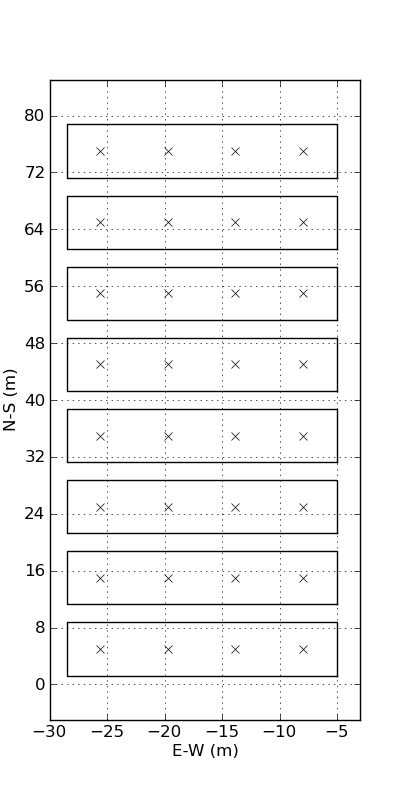
\includegraphics[scale=0.6]{graphics/layout.png}
    \label{fig:ant_layout}
    }
    \hspace{10pt}
    \subfloat[BEST-2 is a subset of eight cylinders in the north-south arm of the Croce del Nord.]{
    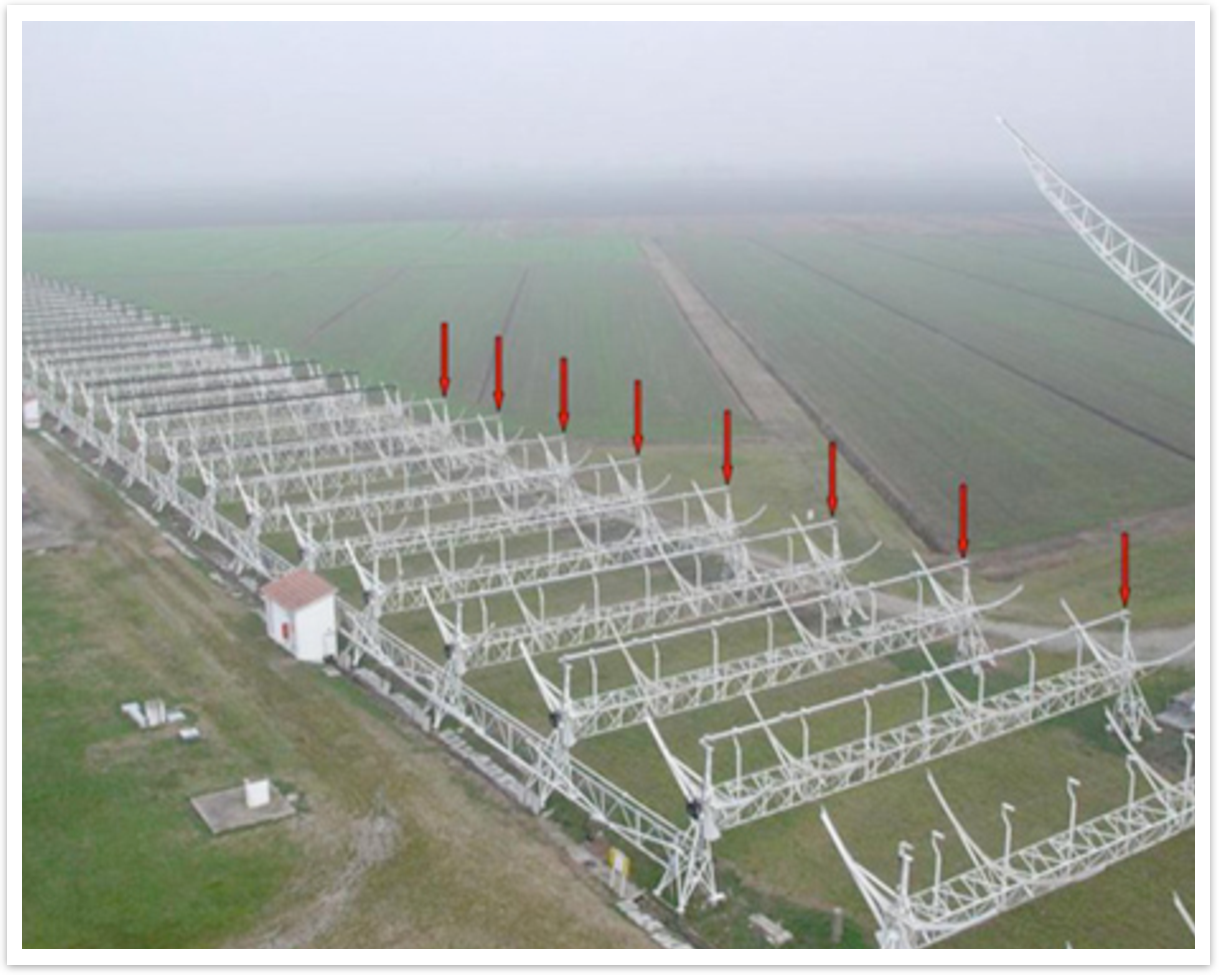
\includegraphics[scale=0.4]{graphics/best2.pdf}
    \label{fig:best2}
    }
    \label{fig:array_layout}
\end{figure}

\section{Instrument Design}
\label{instrument design}

An FX correlator and spatial FFT imager instrument have been built for BEST-2.
Both instruments use the same digitization and channelization frontend.
This allow a streamlined process of calibrating the spatial FFT imager, reduces the amount of hardware and allows for simultaneous observation with both instruments.
The instrument has been implemented on ROACH boards which are a generic field programmable gate array (FPGA) board designed by CASPER for radio astronomy applications.
A ROACH consist of a XILINX Virtex 5 SX95T FPGA with interfaces to DRAM and QDR memory, high speed CX-4 connectors and a generic Z-DOK interface for connecting ADCs and various daughter boards, fig \ref{fig:roach}.
Additionally, the board has a PowerPC running BORPH, a variant of Debian Linux, which allows access to software registers and shared memory on the FPGA.
Firmware is designed using MATLAB Simulink which is extended with XILINX DSP blocks and CASPER's open source DSP blocks\footnote{https://casper.berkeley.edu/}.
Design specific DSP blocks and hardware interfaces have also created, design models and control software are available from our project repository\footnote{https://github.com/griffinfoster/medicina}.
Instrument design specifications are presented in table \ref{tbl:digital_specs}, further design detail is described in the following sections.

\begin{figure}
    \centering
    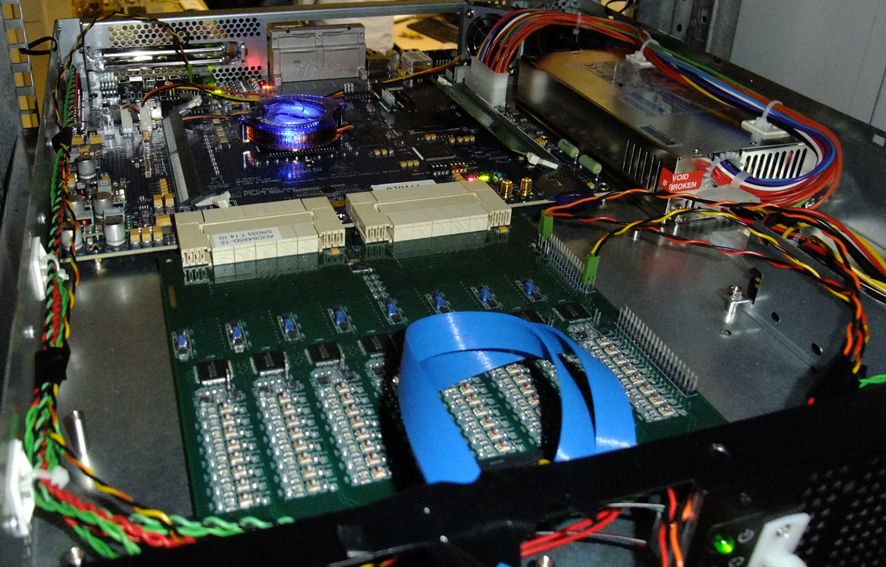
\includegraphics[scale=0.4]{graphics/roach_feng.png}
    \caption{The 'f-engine' ROACH board, a Virtex 5 SX95T FPGA board, with the 64 input ADC connected via two Z-DOK connectors.}
    \label{fig:roach}
\end{figure}

\begin{table}
\begin{center}
\begin{tabular}{| l | l | l |}
\hline
\multicolumn{3}{|c|}{Digital Backend Specifications}\\
\hline
Digitizer/Channelizer (F-Engine) & &\\
\hline
ADC Sampling Rate	& 40 			& MHz\\
ADC Sampling Precision	& 12 			& bit \\
Antenna-polarizations 	& 32 			& single pol \\
PFB 			& 4 tap FIR + 2048 point FFT	& Radix-2 Biplex Real FFT\\
Quantization 		& 4 			& bit\\
& & \\
\hline
FX Correlator (X-Engine) & &\\
\hline
Auto Correlations 	& 32 			& \\
Cross Correlations 	& 496 			& \\
Minimum Integration Length & 6.55 		& ms\\
Output 			& 10 GbE 		& SPEAD protocol\\
& & \\
\hline
Spatial FFT Imager (S-Engine) & &\\
\hline
2D FFT 			& 8 x 16 		& \\
Beams 			& 128 			& \\
Minimum Integration Length & 1 			& s\\
Output 			& 1 GbE 		& SPEAD protocol\\
Beamformer Output 	& 10 GbE 		& Up to 8 Beams\\
& & \\
\hline
\end{tabular}
\caption{A three ROACH design where the correlator and spatial FFT imager use the digitizer/channelizer interface.}
\label{tbl:digital_specs}
\end{center}
\end{table}

\subsection{Digitization and Channelization}
\label{channelization}

Signal digitization is performed using the Texas Instruments ADS5272 8 channel, 12 bit ADC.
The ADC board, developed by Rick Raffanti \footnote{https://casper.berkeley.edu/wiki/64ADCx64-12}, uses eight of these ADCs to channelize 64 streams at up to 65 Msps.
In our design only 32 signal streams are digitized at 40 Msps which more then covers the 16 MHz analog band.
The ADC is clocked with a 160 MHz clock which is locked to a local maser source.
During the analog stage the RF, centered at 408 MHz, has been mixed down to baseband.
Prior to digitization the last amplifier stage of the analog chain has per signal adjustable gain useful for setting good levels for ADC quantization.
This ADC is connected via a dual Z-DOK interface to an 'F-Engine' ROACH which performs the channelization.
The ROACH board is clocked at four times the sample rate such that four signals are time division multiplexed onto a single stream.
Channelization is performed with a four tap Hann filter, 2048 point polyphase filterbank (PFB) to produce 1024 samples per real antenna stream.
The CASPER PFB has been modified to account for the signal multiplexing.
Each channel has a width of 19.5 kHz and the output of the FFT stage is a 36 bit complex number.
The narrow channel widths and PFB windowing allows for good frequency separation in the high RFI environment at the observatory.
After channelization the samples are quantized down to a 8 bit complex number.
An adjustable, per channel complex gain equalizer is used for amplitude and phase corrections before quantization.
Complex gain calibration is essential to proper spatial FFT imaging which must be applied before the spatial FFT.
The FX correlator is used to generate calibration coefficients which are applied back into the equalizers.
A selectable mux is available to skip the phase coefficients on the FX correlator data stream.
Post equalization the data stream is split into two for specific reordering for the correlator and imager.
The correlator data stream is reordered to 128 time samples for a single antenna for a single frequency channel.
Followed by the next antenna and cycles back onto the next frequency channel.
The imager takes in one time sample of each antenna for a given frequency channel and cycles through 128 time samples before stepping to the next frequency channel.
After data reordering each stream is sent over high speed XAUI at a rate of 5.12 Gbps to the correlator and imaging boards.

\begin{table}
\begin{center}
\begin{tabular}{| l | l | l |}
\hline
\multicolumn{3}{|c|}{F-Engine ROACH Resource Utilization (Virtex 5 SX95T)}\\
\hline
ADC Clock 		& 40 MHz \\
System Clock 		& 160 MHz 	& Demux:4 \\
Slice Registers 	& 30217 / 58880 & $51\%$\\
Look Up Tables 		& 24319 / 58880 & $41\%$\\
BRAM (36kb) 		& 205 / 244 	& $84\%$\\
DSP48e (Multipliers) 	& 185 / 640 	& $28\%$\\
CX-4 Interface 		& 2 / 4 	& 5.12 Gbps XAUI\\
QDR Memory 		& 2 / 2 	& Cornerturn\\
\hline
\end{tabular}
\caption{DSP implementation of the 'f-engine'}
\label{tbl:feng_resource}
\end{center}
\end{table}

\begin{figure}
    \centering
    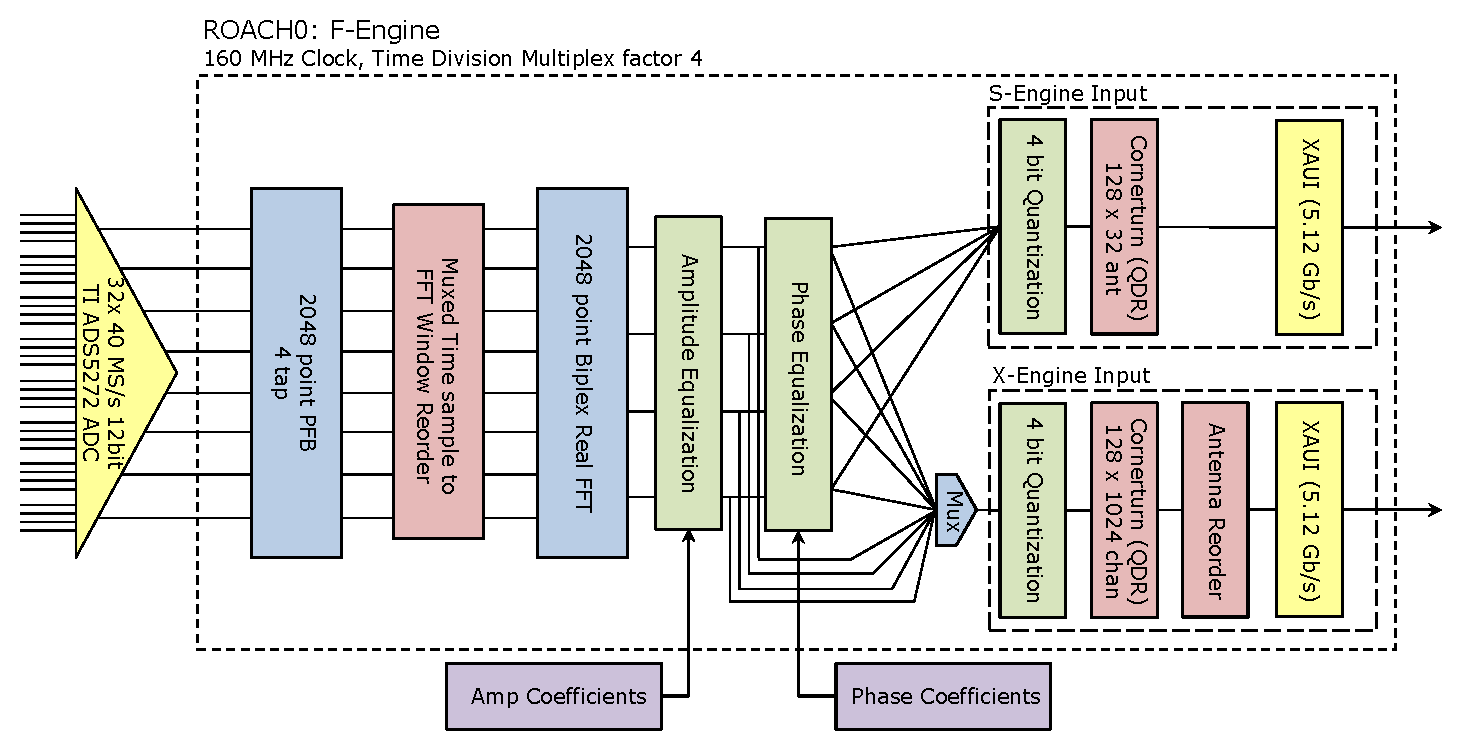
\includegraphics[scale=0.6]{graphics/crop_fengine_block.pdf}
    \caption{During observations amplitude and phase coefficients are applied to scale the power for the 4 bit correlation and apply phase corrections for the spatial FFT.}
    \label{fig:feng_block}
\end{figure}

\subsection{FX Correlator}
\label{correlator}

An FX correlator design is a standard design for large bandwidth and many antenna arrays.
The F component represents the frequency channelization, and the X is a complex multiply and accumulate (CMAC).
An overview of the architecture is presented in \citep{}.
Architecture efficiency goes as $O( M \textrm{log} M) + O( N^2)$ where $M$ is the number of FFT frequency channels and $N$ is the number of antenna-polarizations.
The core component to the X stage of the FX correlator is the complex multiplication of all pairs of independent signals for each frequency channel.
A pipelined x-engine, based on the general CASPER block originally designed by Lynn Urry\citep{}, is used for multiplier efficiency.
The pipeline design is constructed out of $M/2$ 'taps' where the $i^{th}$ tap computes the correlation between antennas $A_j$ and $A_{j+i}$ for every antenna $A_j$ of $M$ total antennas.
To maximize the multiplier usage a loopback is added to use every $i^{th}$ tap to compute the correlation of antennas $A_j$ and $A_{M/2+j+i}$, fig. \ref{fig:xeng_pipe}.
Each tap accumulates for $N$ time samples to reduce the output data rate.

\begin{figure}
    \centering
    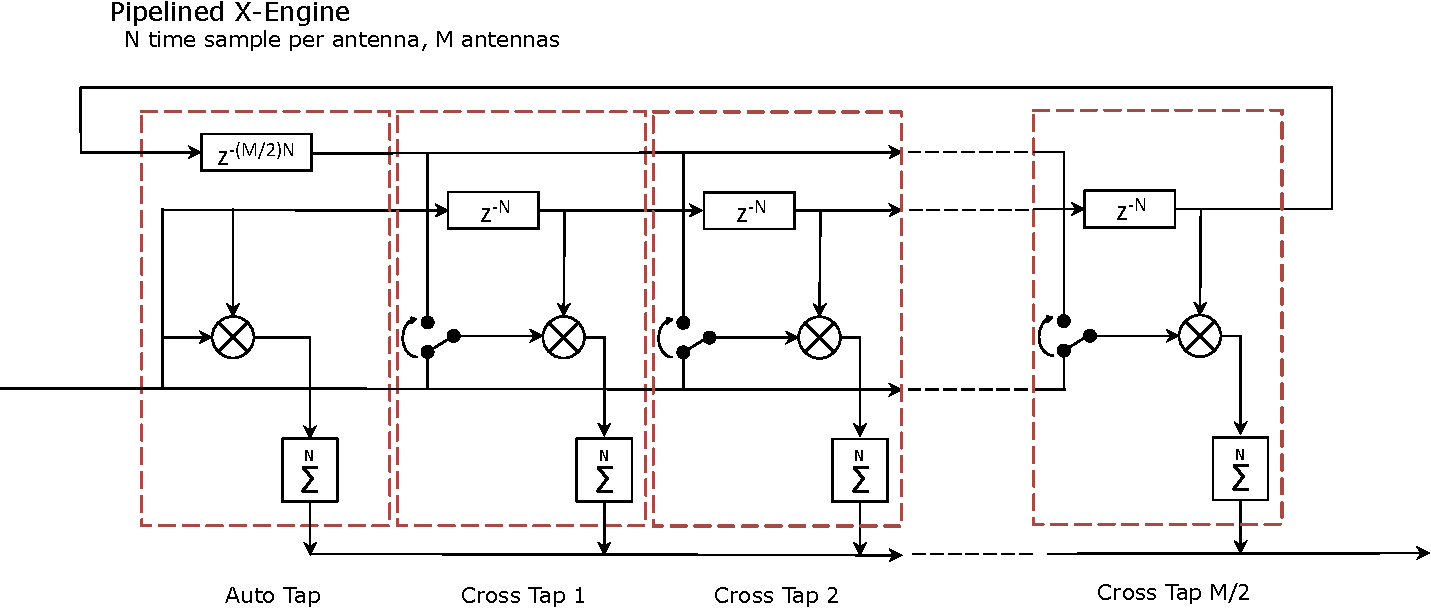
\includegraphics[scale=0.6]{graphics/crop_pipelined_xeng.pdf}
    \caption{The input is ordered as $N$ time samples per antenna per frequency channel. An accumulation stage after the complex multiply reduces the data rate of each tap. Outputs are multiplexed onto the same output using a valid signal.}
    \label{fig:xeng_pipe}
\end{figure}

An asynchronous architecture is used between the f-enigne and x-engine boards.
The x-engine board has been clocked to 200 MHz, well above the 160 MHz f-engine board, this assures the x-engine board will never have input buffer overflows during the windowing stage.
The XAUI interboard connection is a streaming interface which guarantees the same output order as input order but with variable latency.
In rare cases the XAUI interface can drop 64 bit words during the streaming, this requires an initial stage to track the number of words received between headers.
In case of missing words the entire payload is dropped and counters reset for the next header.
A correlation is only performed on a per channel basis.
The channelized band can be split up into portions and processed in parallel across multiple x-engines.
This allows a larger bandwidth to be processed at the cost of increased logic and multiplier resource utilization.
For this design two x-engines are used which each processes half of the band.
The x-engine design requires a continuous stream of data for 128 samples of all antennas for a single frequency channel.
Prior to the x-engine samples are buffered up into windows to guarantee valid data during a cycle of the x-engine.
For reasons related to the design the 32 single polarization signals are treated as 16 dual polarization signals.
This causes a small number of redundant baseline correlations and a conjugation effect which is corrected in post processing.
During the x-engine stage an initial accumulation of 128 sample is performed after the complex multiply to reduce the output rate to roughly the input rate.
This limits the minimum integration time to 6.55 ms.
In addition to the standard CASPER pipelined x-engine design an optimized version has been tested.
This new optimized design efficiently uses the full bit width of the Xilinx DSP48 multipliers to reduce the total multiplier usage by a 75\%.
A full description of this design is in preparation.
A vector accumulator using the on board QDR memory is used for longer integration lengths.
This second accumulator is software controlled with integration lengths ranging from milliseconds to minutes.
A completed integration is sent to a receive computer over a 10 GbE connection.
Integrations are split up based on the SPEAD protocol\footnote{https://github.com/ska-sa/PySPEAD} and transmitted as UDP packets.

\begin{table}
\begin{center}
\begin{tabular}{| l | l | l |}
\hline
\multicolumn{3}{|c|}{X-Engine ROACH Resource Utilization (Virtex 5 SX95T)}\\
\hline
System Clock & 200 MHz \\
Slice Registers & 28494 / 58880 & $48\%$\\
Look Up Tables & 25349 / 58880 & $43\%$\\
BRAM (36kb) & 88 / 244 & $36\%$\\
DSP48e (Multipliers) & 288 / 640 & $45\%$\\
CX-4 Interface & 1 / 4 & 5.12 Gbps XAUI\\
QDR Memory & 2 / 2 & Vector Accumulator\\
\hline
\end{tabular}
\caption{DSP implementation of the 'x-engine'}
\label{tbl:xeng_resource}
\end{center}
\end{table}

\begin{figure}
    \centering
    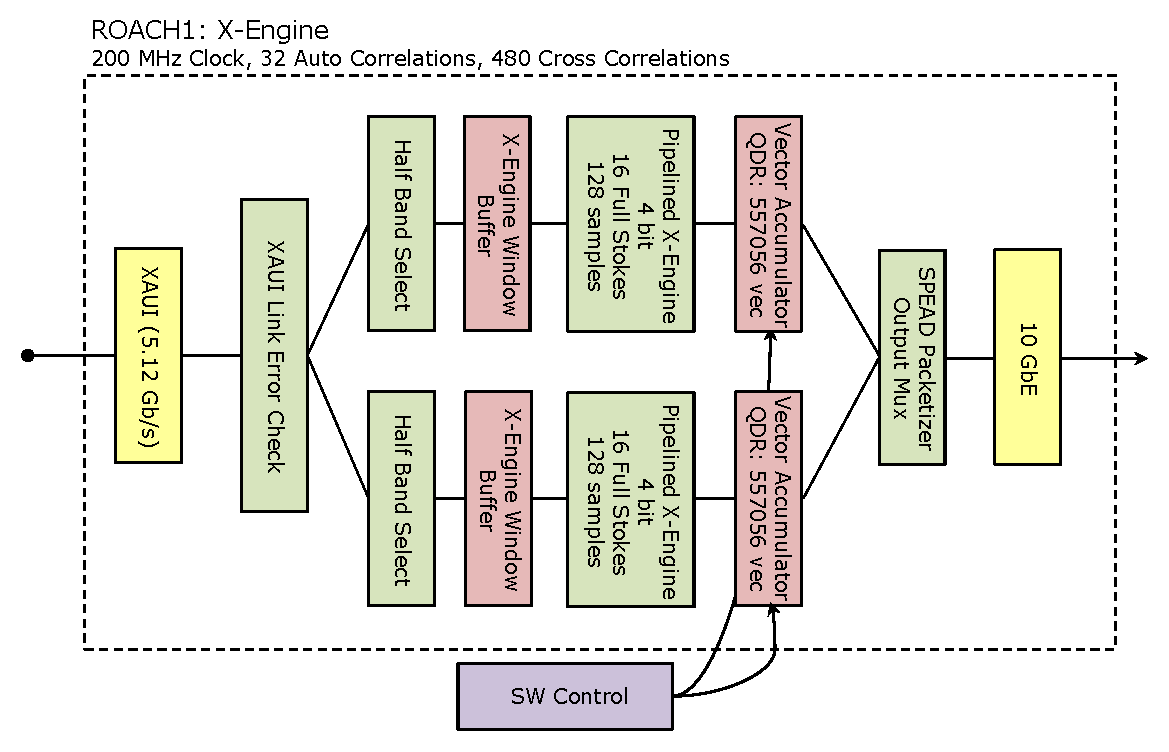
\includegraphics[scale=0.6]{graphics/crop_xengine_block.pdf}
    \caption{Two parallel pipelined x-engines are used, each processes half of the band.}
    \label{fig:xeng_block}
\end{figure}

\subsection{Spatial FFT}
\label{s-engine}
 
When $N$ receiving elements in an antenna array are placed on a regularly spaced grid, a well known method for producing a complete set of orthogonal beams on the sky is the spatial fast Fourier transform \citep{fastbeamforming}.
Such a beamforming implementation will generate $N$ beams on the sky, with a computational cost of $O(N\log{N})$. For large arrays, where many beams are desired, this can be a significant computational saving, with the alternative, so-called \emph{DFT beamforming}, requiring $O(N)$ operations per synthesized beam.
To date, the largest such astronomical implementation of such a spatial fast Fourier transform beamformer is the 64 element dish array constructed in 1994 at Waseda University, Japan \citep{2dfft}.

More recently, spatial FFT based processing has been revisited in the literature with an emphasis on the correlation matrix, rather than the collection of beams, as the mathematical object of interest \citep{fftt} \citep{omniscope}.
In the method outlined by Tegmark \& Zaldarriaga, zero padding is applied to the matrix of antenna signals before the spatial FFT is performed, and as such, the complete set of visibilities for all unique baselines in the array can be obtained, post integration, by inverse Fourier transform.
Conversely, in the image plane, the zero-padding required by the prescribed algorithm results in the generation of $~2^{m}N$ beams on the sky and is dependent on the number of dimensions, $m$, in the antenna array.
Regardless of potential downstream visibility domain processing, this oversampling of the sky by a factor $2^{m}$ has the benefit of increasing the instantaneous uniformity of sky coverage by synthesized beams, which somewhat alleviates the limitations associated with the inability to steer multiple beams independently.

%A spatial FFT imager is a novel instrument which takes advantage of the baseline redundancy in a regularly gridded array to reduce the correlator cost of an FX design $O(n^2)$ to a FFT cost of $O(n \log{n})$.
%Correlation of all antenna pairs in a regularly gridded array makes redundant measurements for many of the baselines.
In the BEST-2 backend described here, the requirements on the spatial FFT processor were multifold. Firstly, the system should be capable of generating images on an $O(\mathrm{second})$ timescale, by the method described by \citep{fftt}. Further, the system should be capable of passing formed beams at full bandwidth, i.e. without any accumulation, to downstream time domain processing systems such as the real-time dedispersion engine \citep{dedispersion}. 


This redundancy for the BEST-2 array is show in figure \ref{fig:redbl}.
Instead of making individual correlations of the same baseline as in an FX correlator the correlation of the average of each baseline can be computed.
This optimization realizes on the assumption that each redundant baseline measurement is indeed identical.
Thus any calibration to the complex gains must be applied before the spatial FFT.

\begin{figure}
    \centering
    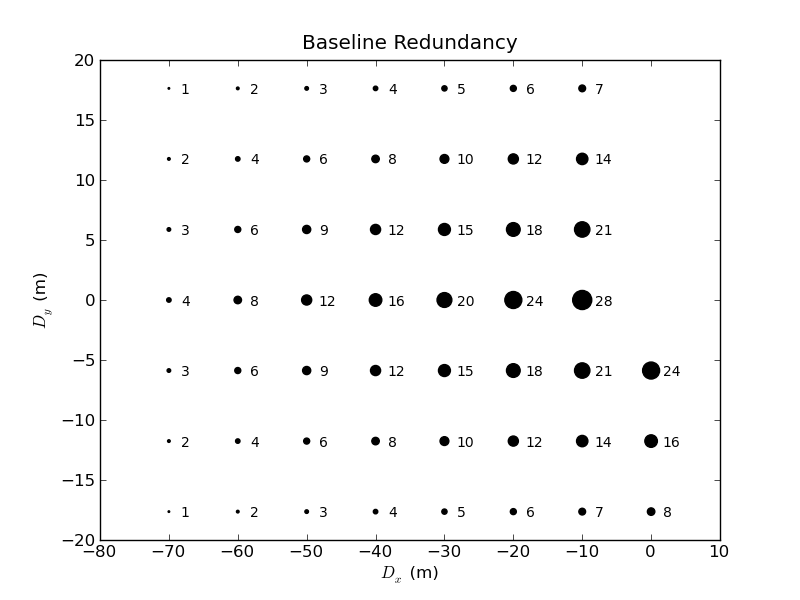
\includegraphics[scale=0.6]{graphics/redbl.png}
    \caption{A 4 by 8 regularly gridded array has 52 unique baselines, 480 cross correlations are performed. The number of redundant baseline measurements is shown as the color and size of each circle.}
    \label{fig:redbl}
\end{figure}

Though the X-Engine and S-Engine use the same F-Engine each requires a unique data windowing order.
For the S-Engine a window is made up of N antennas by M time samples for a given frequency channel.
A similar XAUI interface and windowing scheme is used as in the X-Engine which buffers up windows of valid data to stream into the spatial transform.
The 2D spatial transform is performed using an 8 point FFT followed by a cornerturn and 16 point FFT.
The BEST-2 array is a grid of 4 by 8 antennas, the data is zero padded before input into the 8 by 16 point spatial transform.
A 4 by 8 point spatial transform will only produce gain information for each spatial position, which can be interpreted as an array of beamformers covering the field of view.
This zero padding is necessary to produce both the gain and phase information of each spatial position which is an effective baseline.
Each effective baseline is an average of all possible baselines with the same spatial dimensions.
The four fold increase is the number of outputs from the spatial transform by double padding introduces a number of redundant calculations.
The spatial transform produces 128 outputs, there are only 53 unique baselines in a 4 by 8 grid.
The datarate out of the S-Engine is reduced by a two stage vector accumulator.
A fixed 128 sample vector accumulator reduces the output of the second stage FFT so that the 1024 channels of the 128 computed spatial components can be multiplexed onto one line and accumulated in a software controllable QDR vector accumulator.
Accumulations are sent out over the 1 GbE PowerPC interface using the a SPEAD UDP packet format.
Individual beams can be selected out before accumulation and sent over 10 GbE in a LOFAR beam packet format which will be used for future pulsar processing.

\begin{figure}
    \centering
    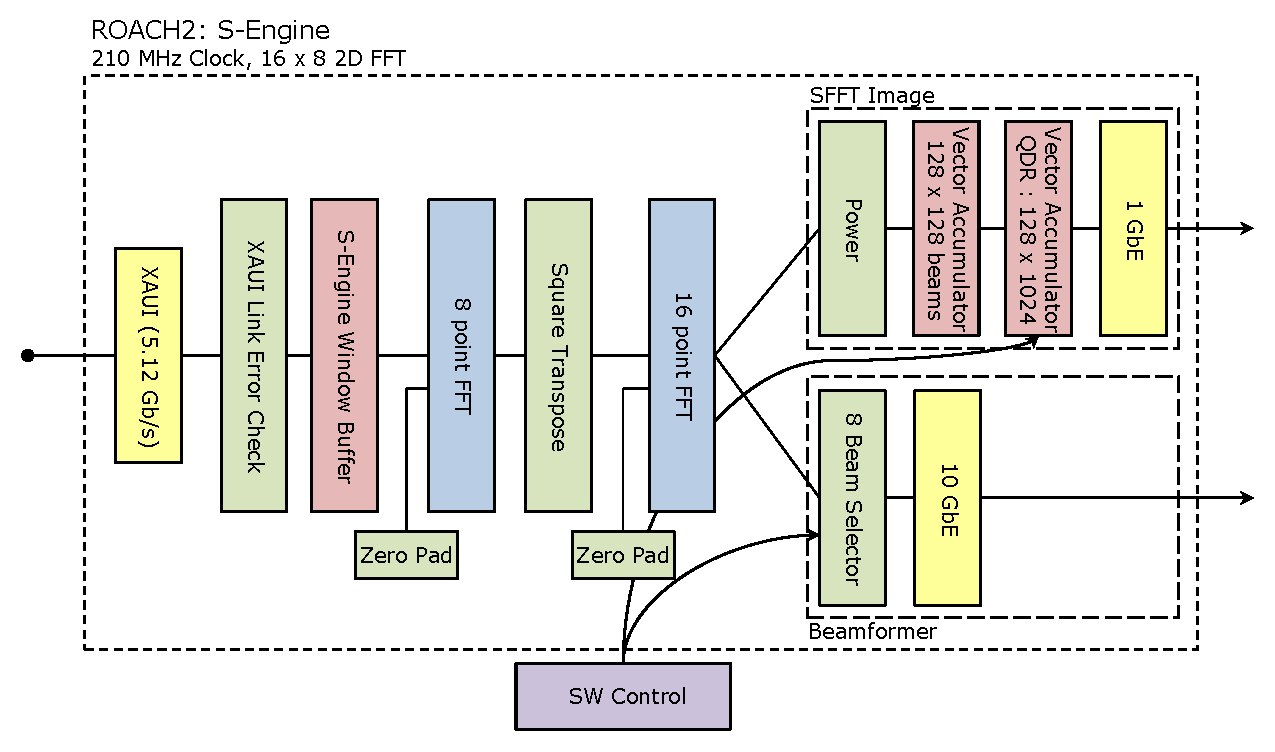
\includegraphics[scale=0.6]{graphics/crop_sengine_block.pdf}
    \caption{During the two stage spatial FFT the streams are zero padded to provide phase information of each baseline.}
    \label{fig:seng_block}
\end{figure}

\section{Deployment and Initial Observations}
\label{observations}

Instrumentation was installed and tested over a two week period in March 2012.
During that time a number of test signals were used to check the system status.
Once the system was checked out various bright radio sources were observed.
Since the Northern Cross is a transiting array there is a limited period of time each day in which a source is with the primary beam.
Bright sources such as Cygnus A, Cassiopeia A and Virgo A also with a number of 3C sources were observed along with multiple constant declination 24 hour cycles were observed.

Raw data from the correlator and imager was recorded to HDF5 files using a SPEAD protocol receive script.
A suite of python scripts have been written to interface and manipulate the data in this pre-calibration stage.
A python FITS-IDI package has been written to convert HDF5 files into the standard FITS format which can be read by AIPS and CASA\footnote{https://github.com/telegraphic/pyfitsidi}.
This allows for conversion to the Measurement Set format which most packages can interface with.

\subsection{Calibration Methods}
\label{calibration}

The effective averaging of redundant baselines in the spatial FFT imager requires complex gain calibrations to be applied during observations.
To derive gain coefficients a calibration method is applied to the FX correlator data.
In initial observations the column ratio gain estimation method from \citep{gaindecomp} was used to compute a per channel, per antenna complex gain term.

%realtime complex gain calibration
%post integration methods

%SFFT correlations of Tau/3c144 before and after calibration
\begin{figure}
    \centering
    \subfloat[Dirty image of Tau/3c144 formed before applying complex gain calibrations in the F-Engine for the spatial FFT.]{
    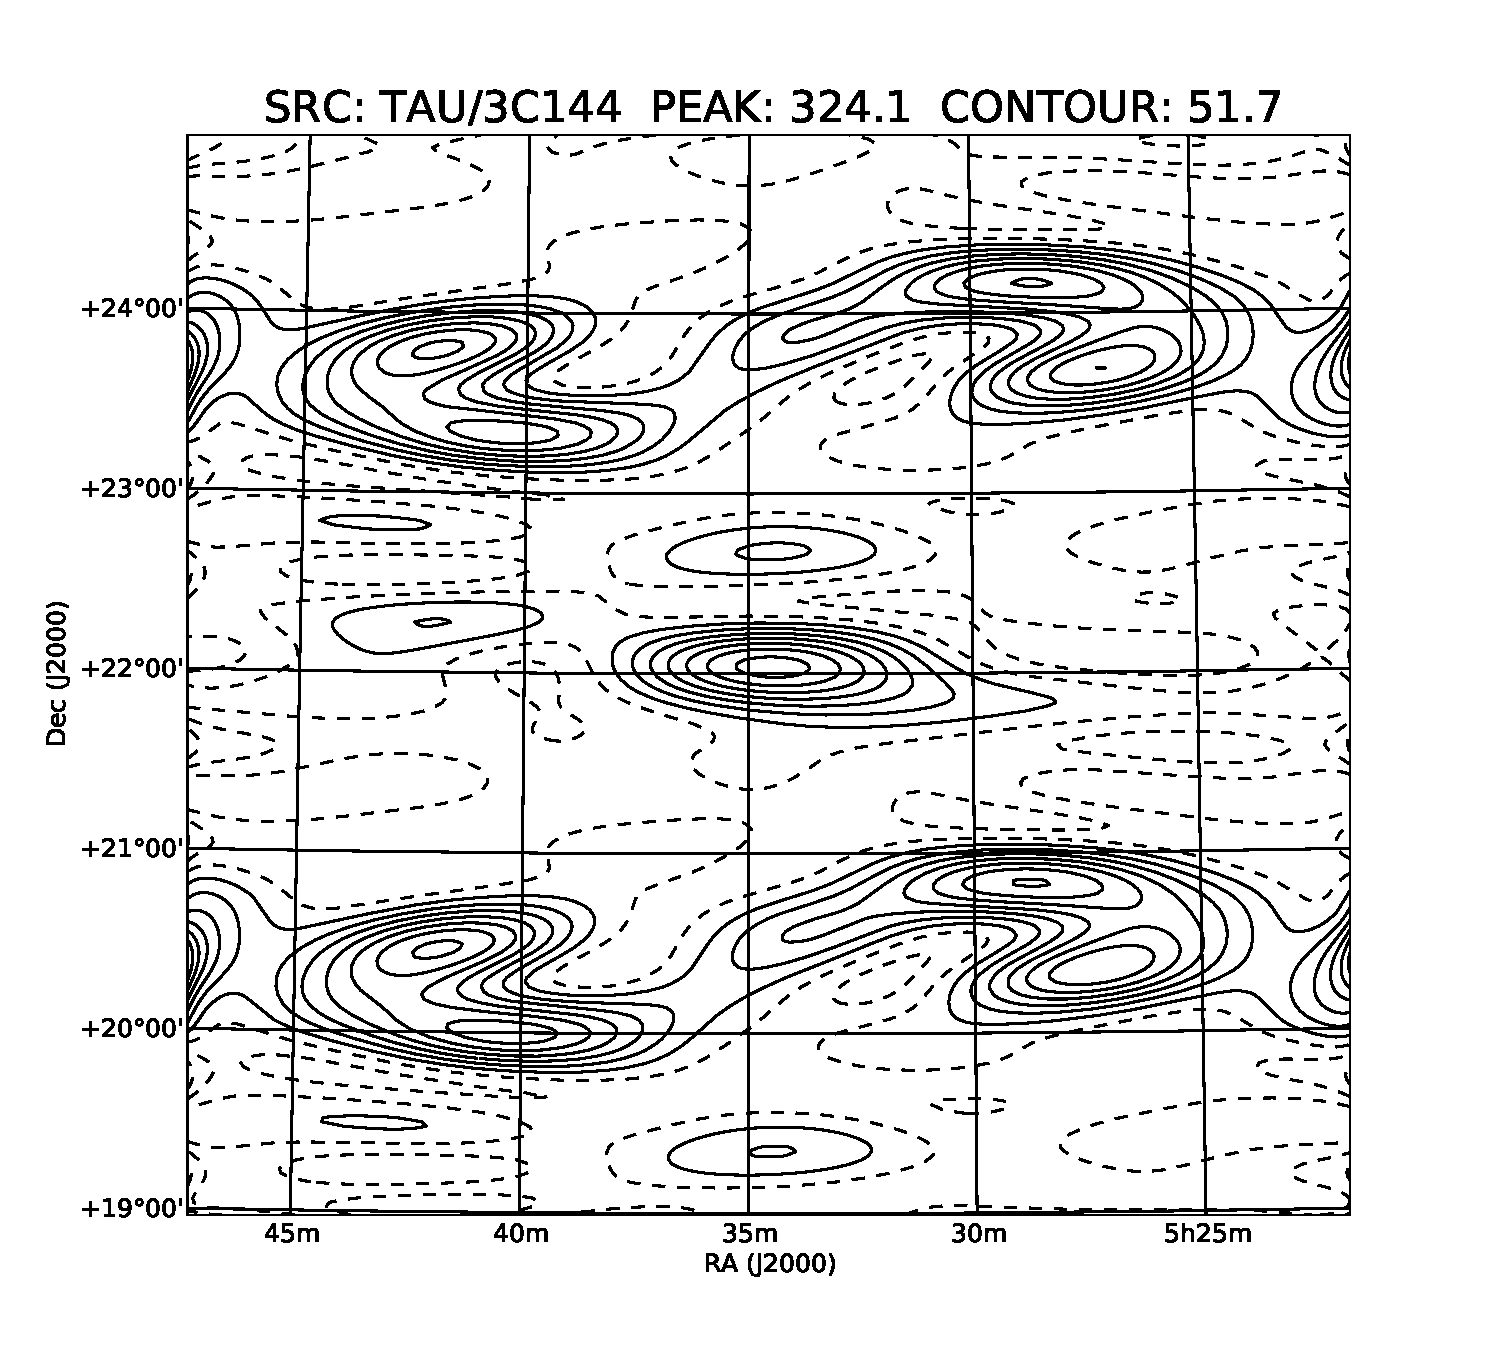
\includegraphics[scale=0.3]{{graphics/img.2455985.25525.tau.uncal.s.ms.DATA.channel.1ch}.pdf}
    \label{fig:uncal_sfft}
    }
    \hspace{10pt}
    \subfloat[Dirty image of Tau/3c144 with complex gain calibrations applied. This image has a signal to noise ratio around 20, a standard CLEAN method can be used to improve the image dynamic range.]{
    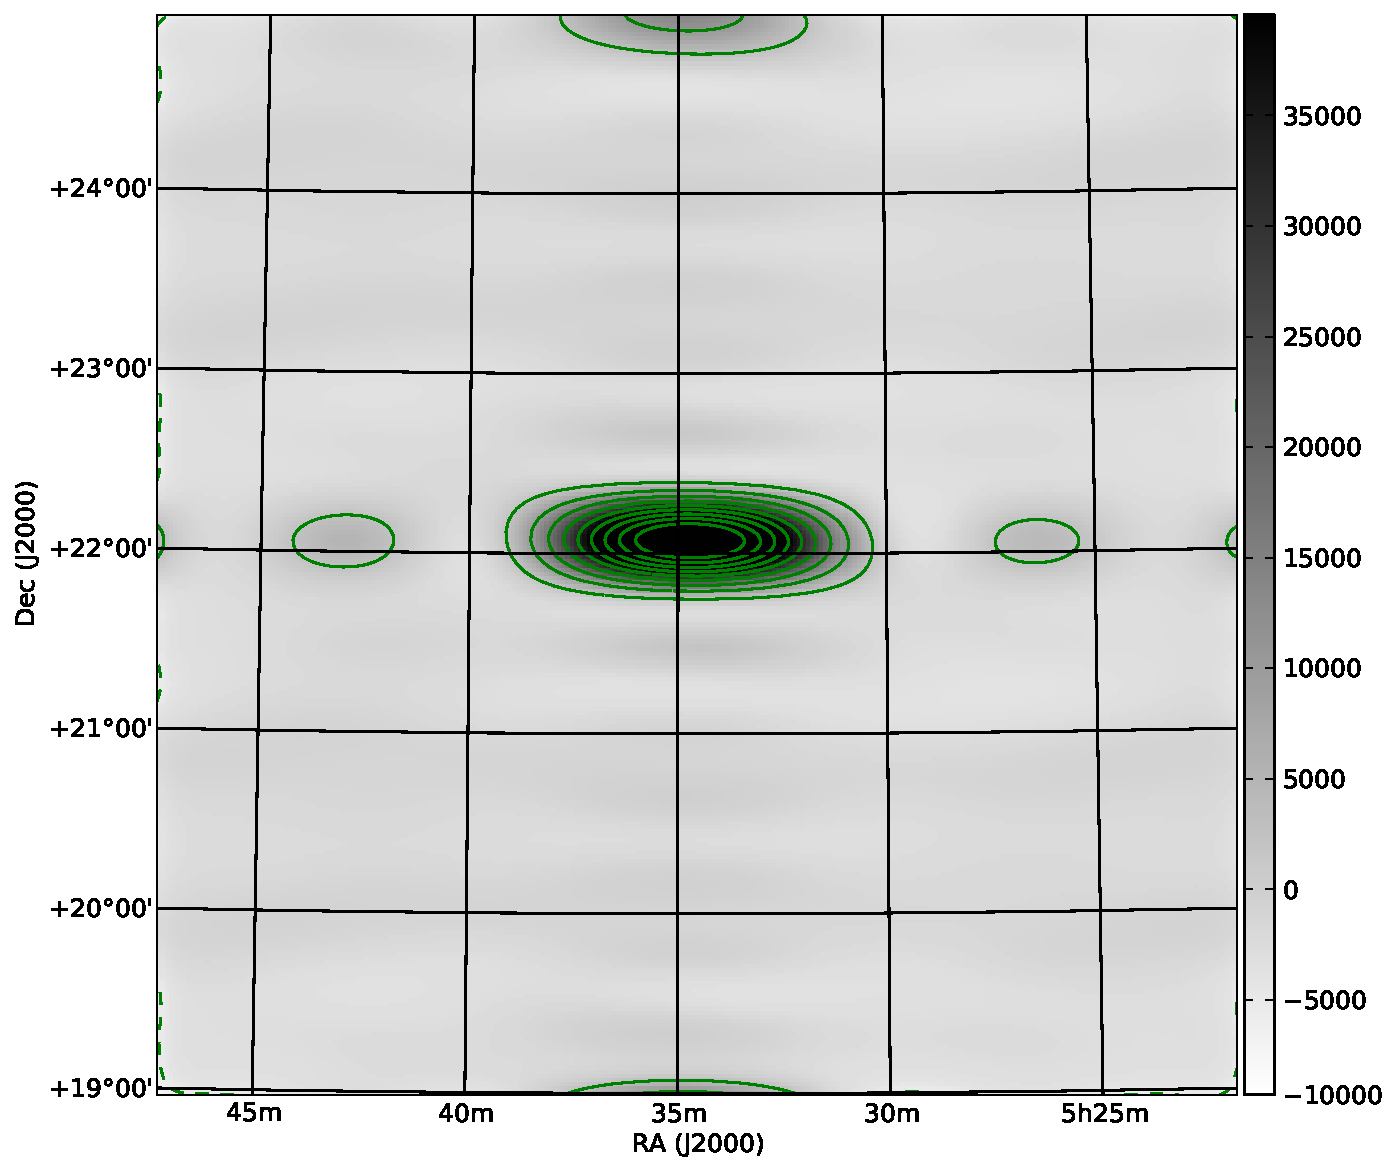
\includegraphics[scale=0.3]{{graphics/img.2455999.21403.tau.cal.s.ms.DATA.channel.1ch}.pdf}
    \label{fig:cal_sfft}
    }
    \label{fig:sfft_calibration}
    \caption{After applying complex gain calibration a bright point source such as Tau/3c144 appears similar to the array psf, and has a significant improvement in the image fidelity compared to the uncalibrated image.
    Scales in both images are based on raw spatial FFT visibilities.}
\end{figure}

\subsection{FX Correlator Imaging}
\label{fx results}

The East-West full width half max (FWHM) beam size of an individual element is $\approx11.25^{\circ}$ which translates to a 45 minute 'transit time' for an source as seen in the measured primary beam, figure \ref{fig:best2_pb}.
For the the bright A class sources this time can be extended since they remain the dominating source well after crossing the FWHM.
Observations of 80-90 minutes are possible which gives an small improvement in uv coverage at the cost of properly accounting for the amplitude modulation due to the primary beam.
This warrants a small sensitivity benefit for a large calibration cost.
Most images are created using data within a few minutes of the source transit time.
The high sidelobes in the primary beam, figure \ref{fig:best2_pb}, cause the bright class A sources to dominate even when they are past their transit time and makes it difficult to perform calibration and imaging near these sources.
During setup intial obseravtions were made of Cygnus A, Cassiopeia A, Taurus A along with a number of 3C sources.

\begin{figure}
    \centering
    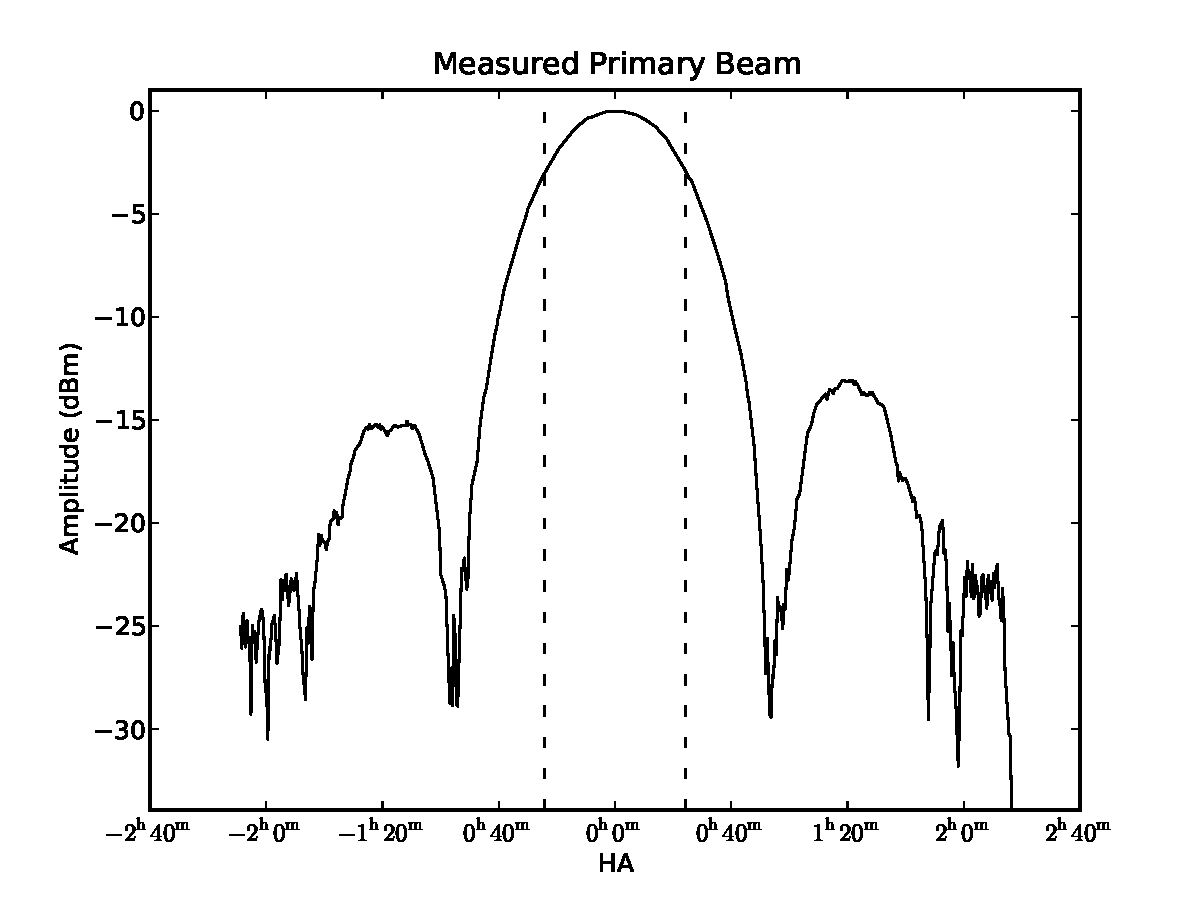
\includegraphics[scale=0.6]{{graphics/pb/best2_3_20_primary_beam}.pdf}
    \caption{Measured east-west primary beam for antenna 1N-6-1, which is representitive of a typical antenna, based on a Cassiopeia A transit. The dashed lines indicate the FWHM points. The first sidelobes are -15 dB down from the peak.}
    \label{fig:best2_pb}
\end{figure}

%calibration/flux scale
A transiting array provides a unique challenge of gain calibration since a source's apparent gain will change as it transits the primary beam.
To account for this a two stage gain calibation method is used.
Phase calibration and setting the flux scale is accomplished using Cas A and Cyg A observations as point source sky models set to their 3C flux levels and known spectral indices.
Since these sources are very bright a only a few seconds at transit is needed produce a high SNR dataset to use for calibration.
Over this period the primary beam can be approximated as flat.
A time independent complex gain is derived for a coarse calibration.
After applying the gain corrections an observation will be set to a flux scale relative to the flux of the calibration source.
Each individual source is further calibrated in MeqTrees\citep{meqtrees} based on a local sky model taken from the 3C catalog.
This stage is calibrated on short time intervals to account for amplitude changes from the primary beam.

%psf/dirty/clean
%dynamic range/noise
An effect of the density of the antenna layout is a low point spread function(PSF) to field of view ratio, or spatial fidelity, thus images tend to contain at most a few spatial seperate point sources.
The grid layout of the BEST-2 array produces strong sidelobes and grating lobes in the PSF as seen in figure \ref{fig:fx_tau_psf}.
Observations of bright point sources produces calibrated dirty images in which the PSF is clearly visible, fig. \ref{fig:fx_tau_dirty}.


%image: raw,psf,dirty,clean
\begin{figure}
    \centering

    \subfloat[Uncalibrated image of Taurus A, the units are raw correlator values.]{
    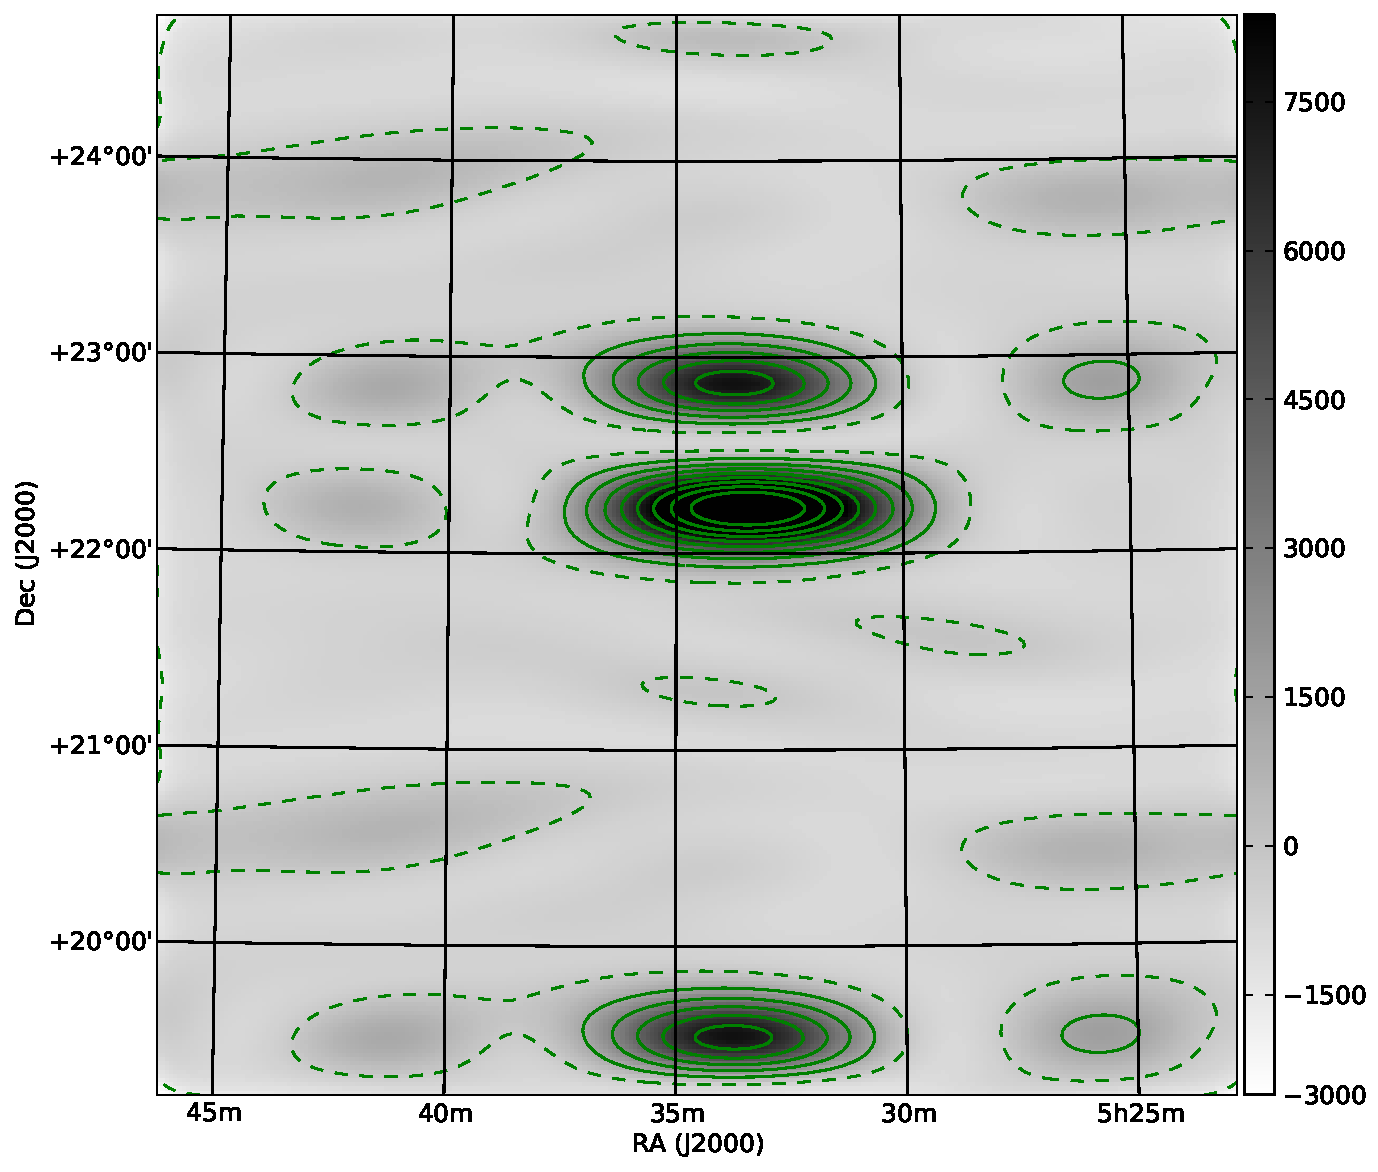
\includegraphics[scale=0.3]{{graphics/fx/corr.2455996.22803.tau.s.ms.DATA.channel.1ch}.pdf}
    \label{fig:fx_tau_data}
    }
    \hspace{10pt}
    \subfloat[Point spread function. The high, regular sidelobes are an effect of the regularly gridded array.]{
    %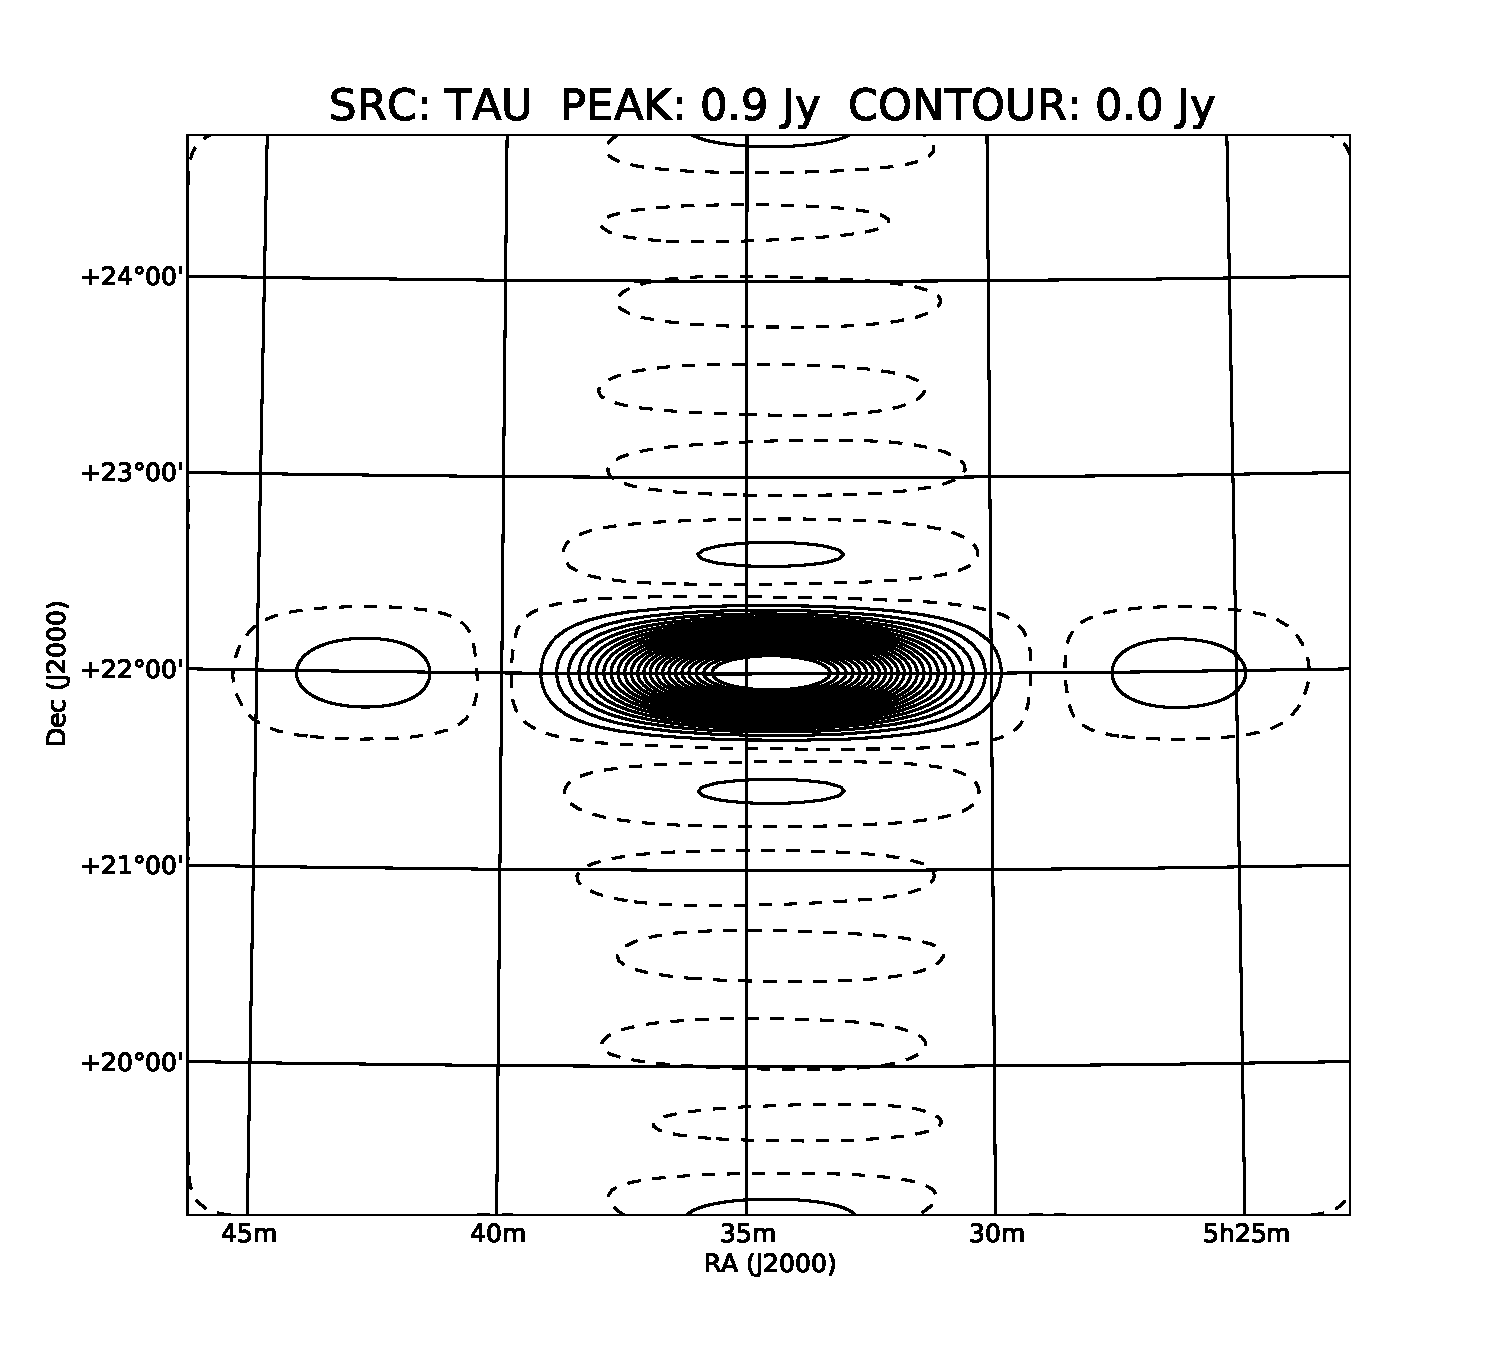
\includegraphics[scale=0.3]{{graphics/fx/corr.2455996.22803.tau.s.ms.psf.channel.1ch}.pdf}
    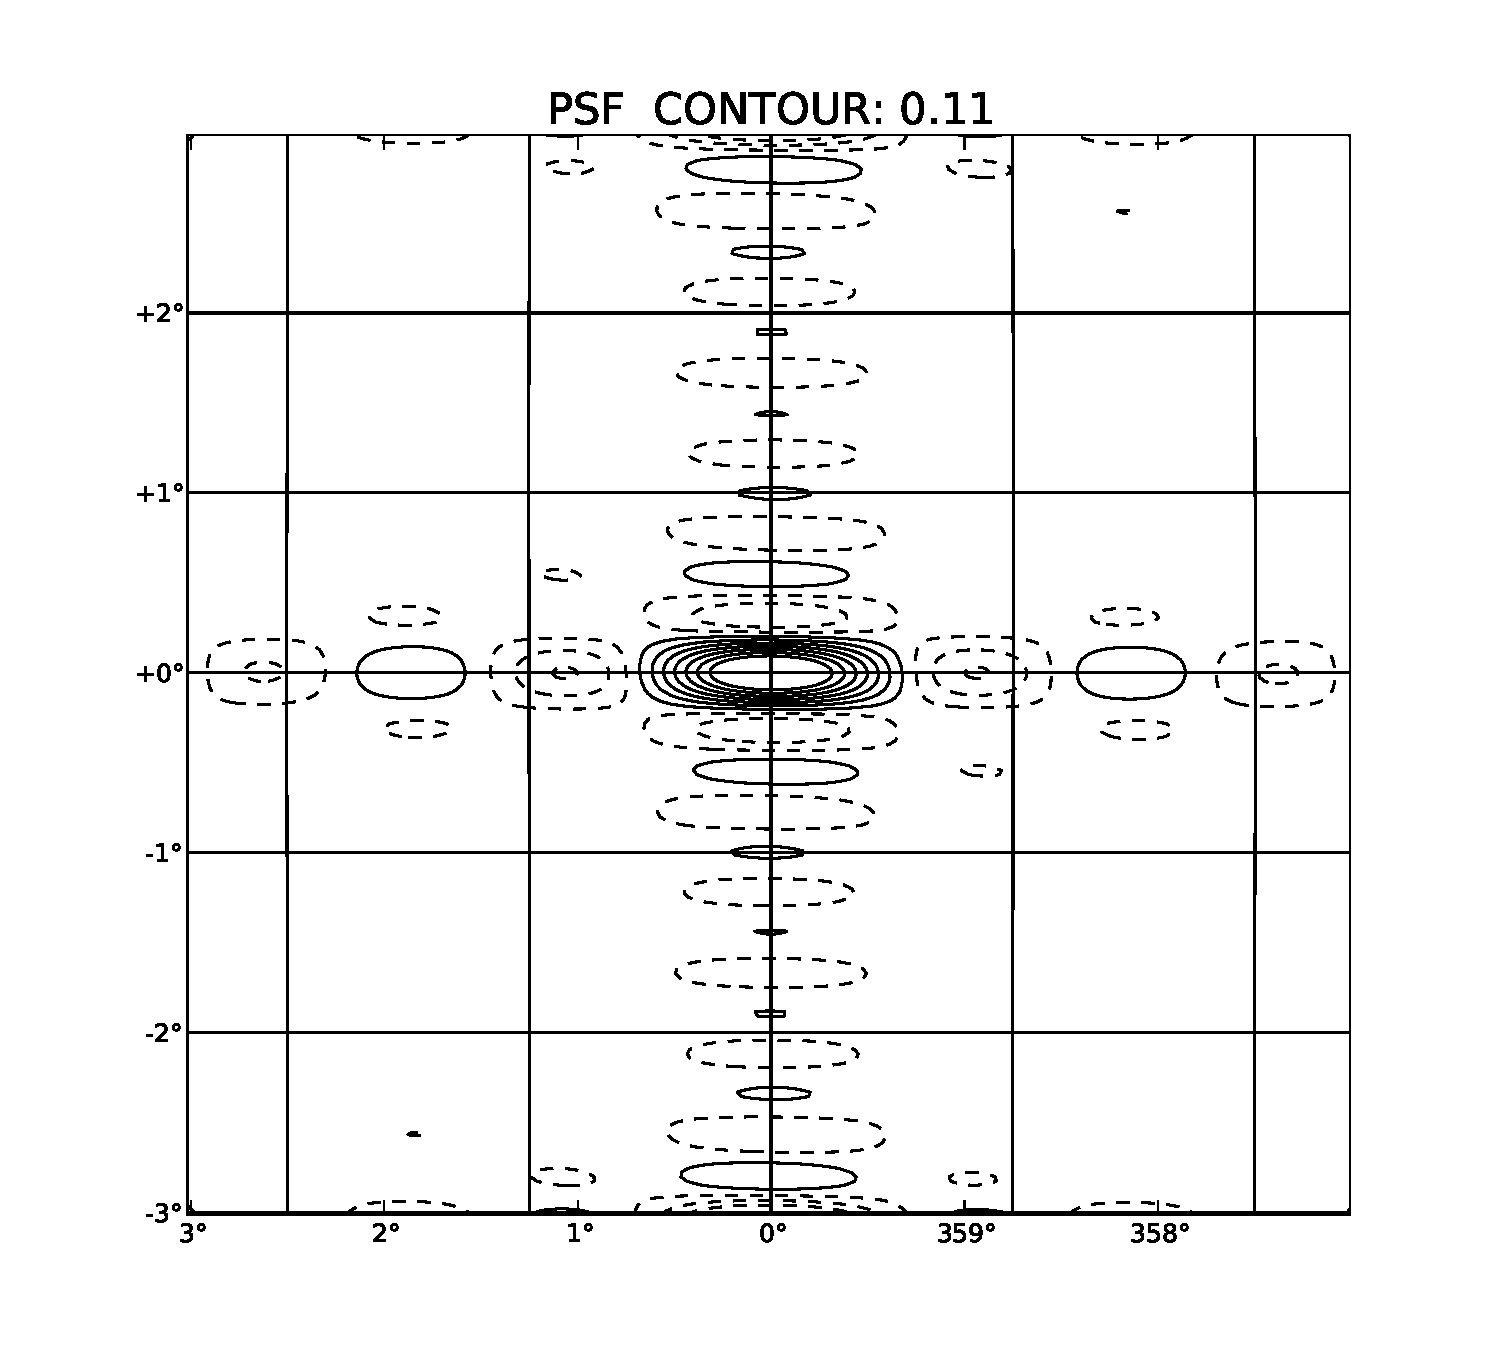
\includegraphics[scale=0.3]{{graphics/img.2455999.21403.tau.cal.s.ms.psf.channel.1ch.mod}.pdf}
    \label{fig:fx_tau_psf}
    }
    
    \subfloat[Image formed, using natural weighting, after applying complex gain solutions. The flux scale(Jy) has been set by the flux of the calibration source.]{
    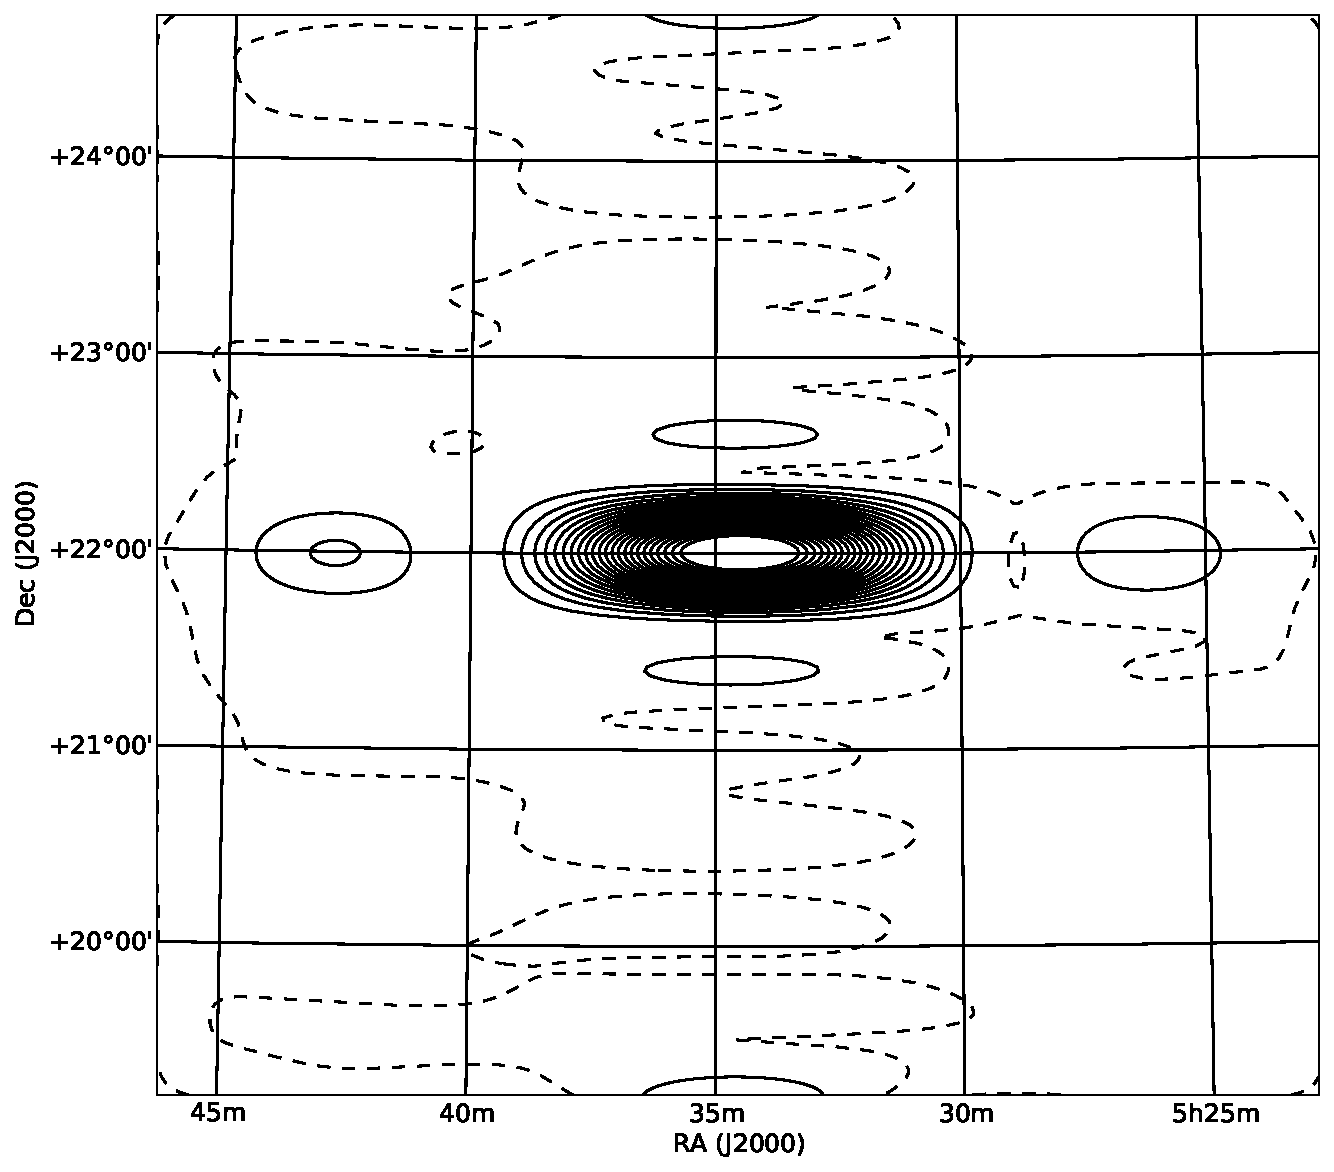
\includegraphics[scale=0.3]{{graphics/fx/corr.2455996.22803.tau.s.ms.CORRECTED_DATA.channel.1ch}.pdf}
    \label{fig:fx_tau_dirty}
    }
    \hspace{10pt}
    \subfloat[]{
    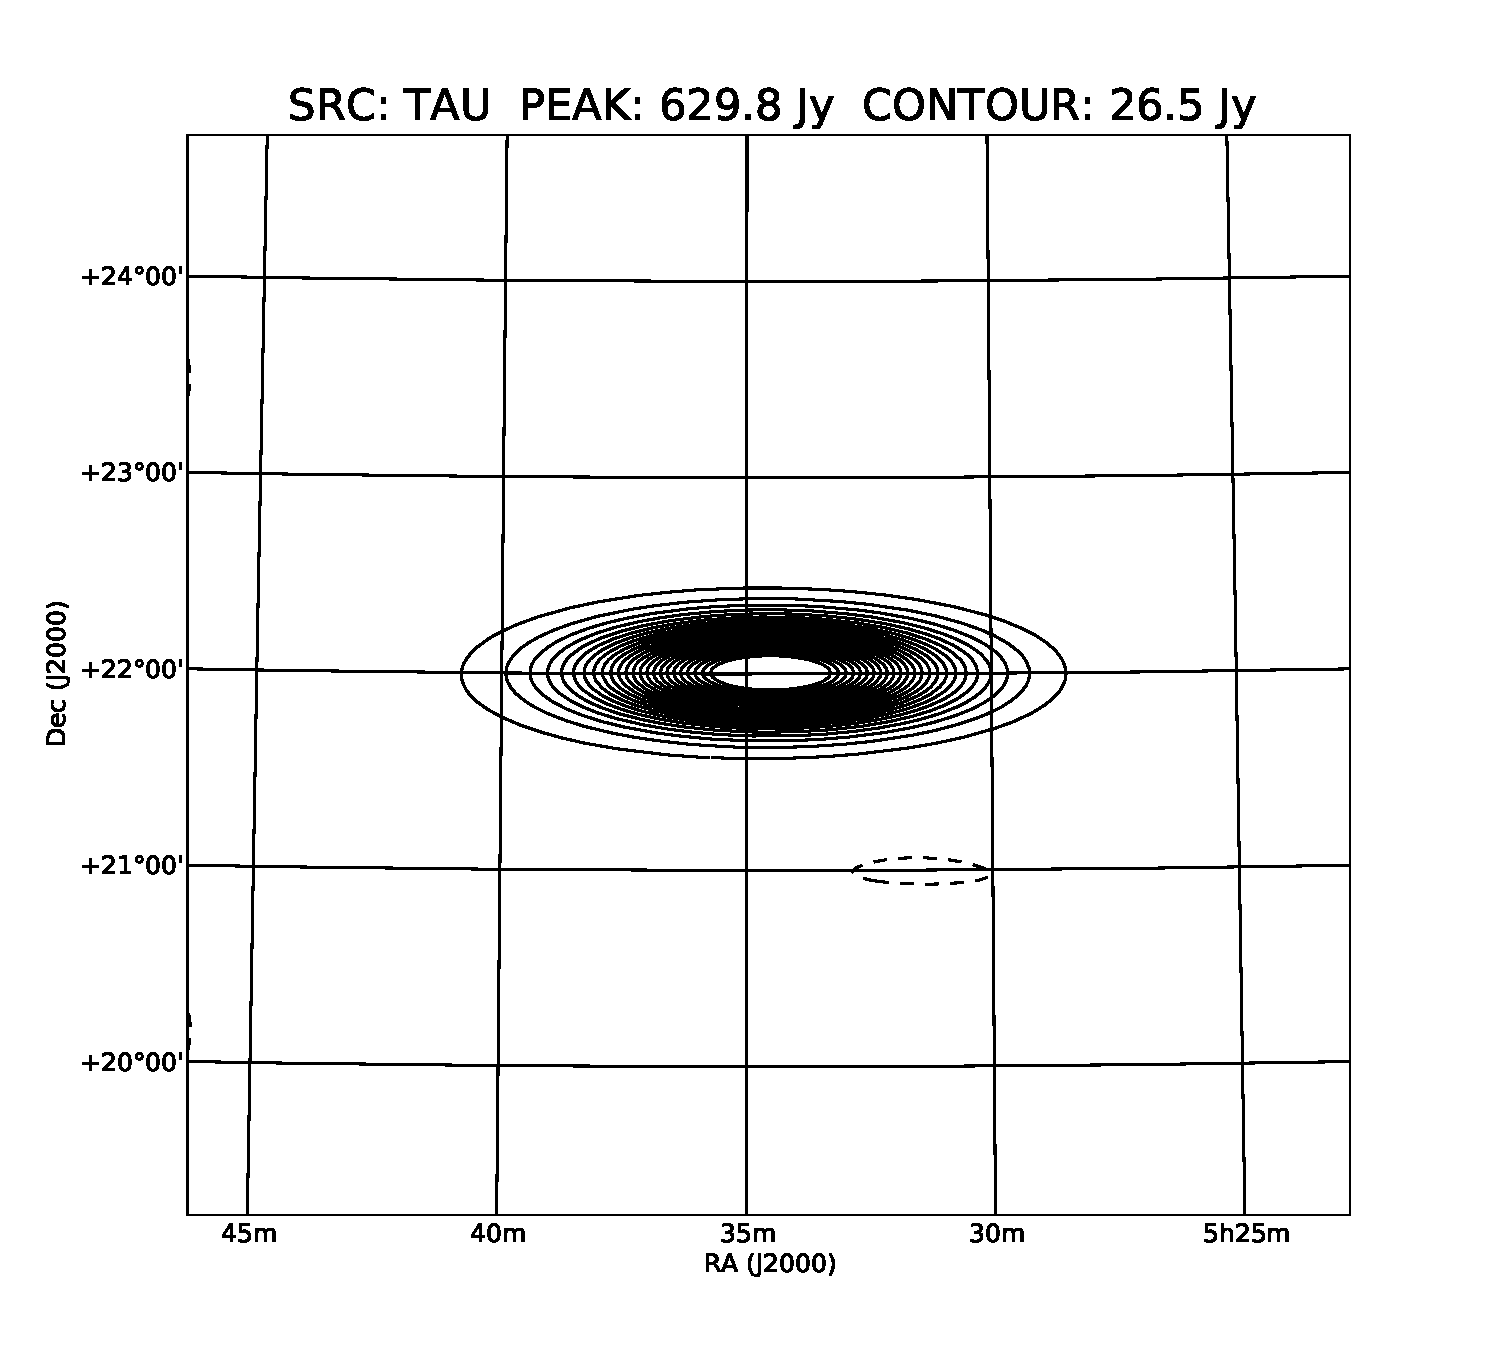
\includegraphics[scale=0.3]{{graphics/fx/corr.2455996.22803.tau.s.ms.CORRECTED_DATA.channel.1ch.restored}.pdf}
    \label{fig:fx_tau_clean}
    }
    
    \label{fig:fx_tau}
    \caption{Images and PSF formed from an FX correlator snapshot observation of Taurus A.
    }
\end{figure}

%solar observation
\subsubsection{Solar Observation during Highly Active Period}

During observations in March 2012 the Sun was at a similar sidereal time as Cassiopeia A.
In that time the Sun was undergoing a very active period.
Even though the Sun was at a declination of approximately $-4^{\circ}$, over $60^{\circ}$ way from Cassiopeia A, the source appears in the same field.
A combintation of high primary beam sidelobes and an active solar period led to the sun being detected $62^{\circ}$ away from it's actual position.
The sun is approximately a half a degree in size, since the longest north-south baseline is about the same size we begin to resolve the sun in that direction.

%image: cas, cas+sun
\begin{figure}
    \centering

    \subfloat[Observation of the Cassiopeia A field on Julian Date 2455985, scale is in Janskys.]{
    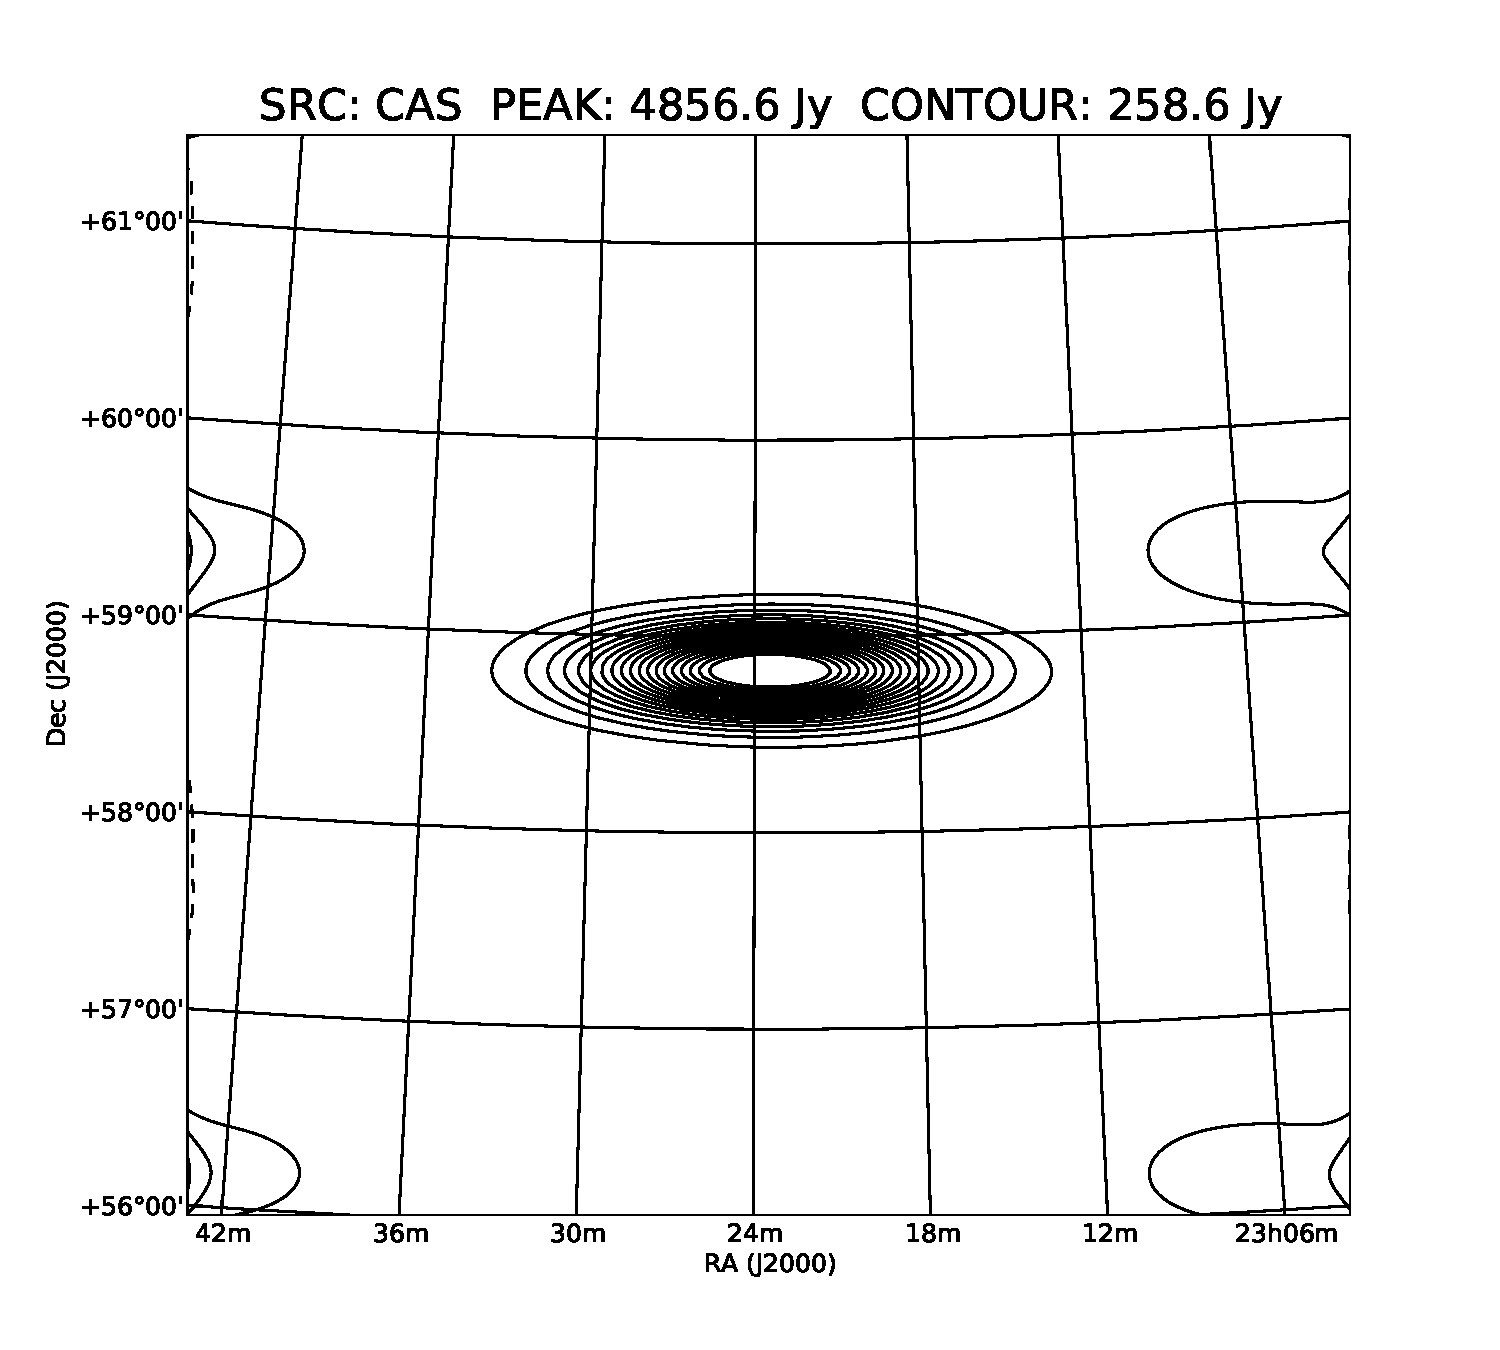
\includegraphics[scale=0.3]{{graphics/fx/corr.2455985.00383.cas.s.ms.CORRECTED_DATA.channel.1ch.restored}.pdf}
    \label{fig:fx_cas}
    }
    \hspace{10pt}
    \subfloat[Observation of the same field ten days later on Julian Date 2455996. The Sun is slightly resolved in the North-South direction. The sun is at declination $-4^{\circ}$, about $62^{\circ}$ from the field of view but is within one of the primary beam sidelobes and has an apparent declination position at $58^{\circ}$.]{
    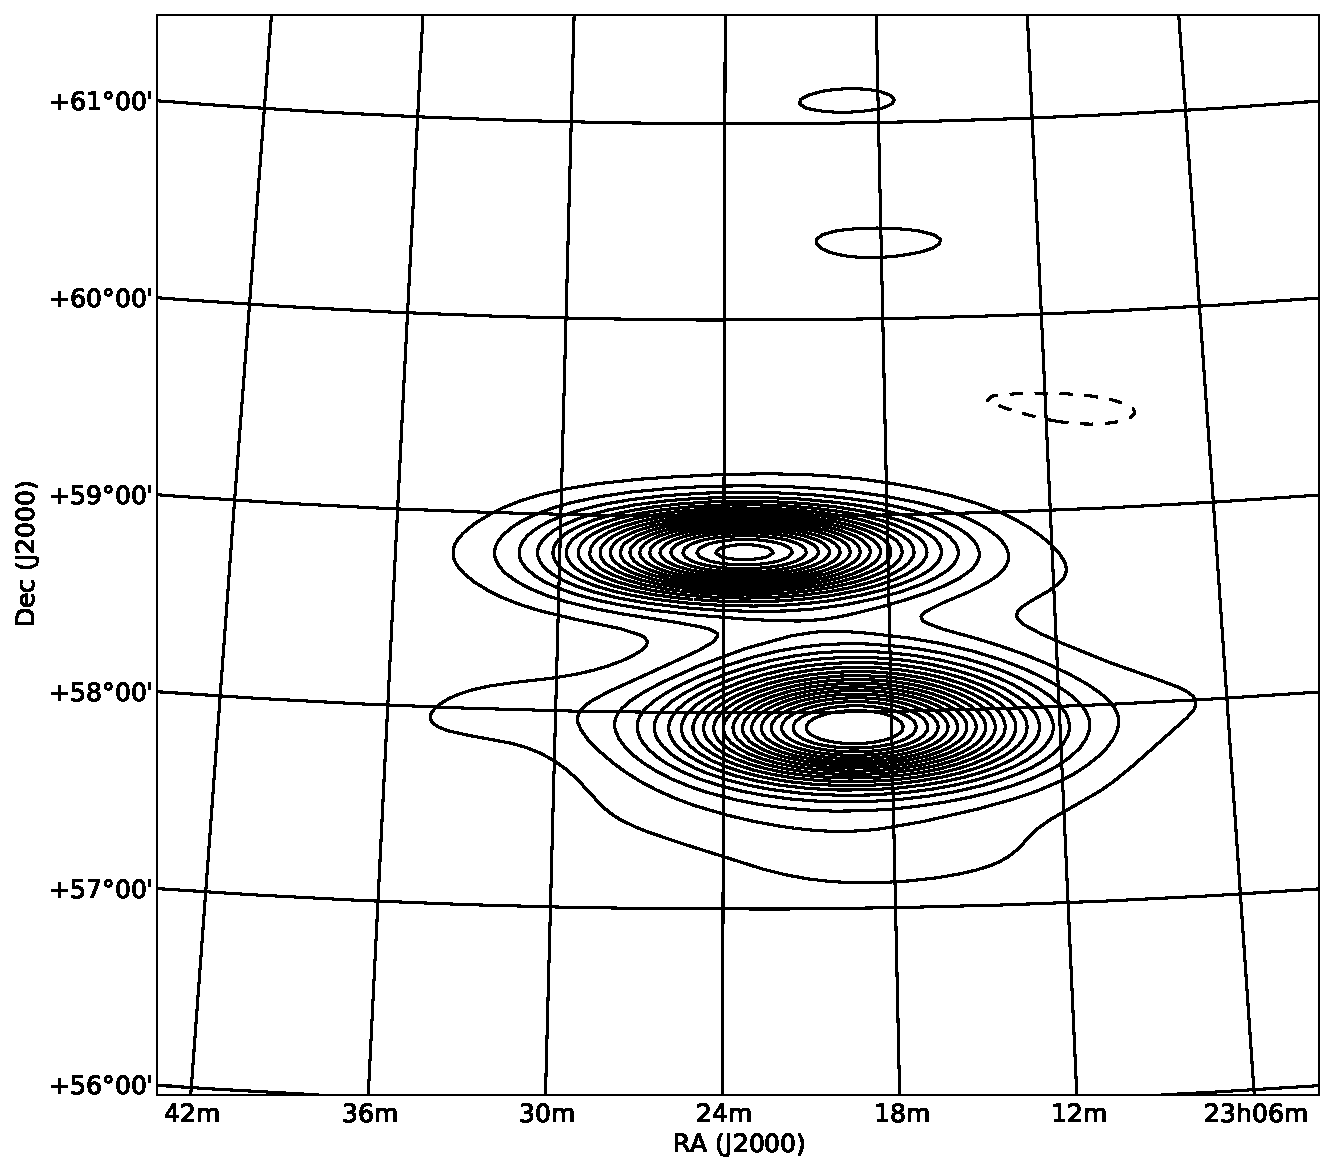
\includegraphics[scale=0.3]{{graphics/fx/corr.2455995.97200.cas.s.g.ms.CORRECTED_DATA.channel.1ch.restored}.pdf}
    \label{fig:fx_cas_sun}
    }
    
    \label{fig:fx_cas}
    \caption{
    }
\end{figure}

%weighting
\subsubsection{Weighting for a Regularly Gridded Array}

As noted earlier, the regular gridded array produces many highly redundant baselines.
When forming the dirty image from uv samples the choice of weighting greatly effects the outcome of the image.
In the highly redundant array case of BEST-2 the effects of using uniform versus natural weighting can be seen in fig. \ref{fig:fx_weighting}.
The uniform weighting scheme significantly reduces the sensitivity the image for a small improvement in spatial resolution.
We have used a natural weighting scheme through out to produce images.
It is worth noting that the baselines produced by the spatial FFT instrument are already in a 'natural' weighting scheme since all redundant baselines are effectively summed together into a single baseline.
To change the weighting of the spatial FFT baselines reweighting factors must be added to the data based on how redundant each baseline is.

%image: natural,uniform
\begin{figure}
    \centering

    \subfloat[Dirty image with natural weighting of the point source Taurus A.]{
    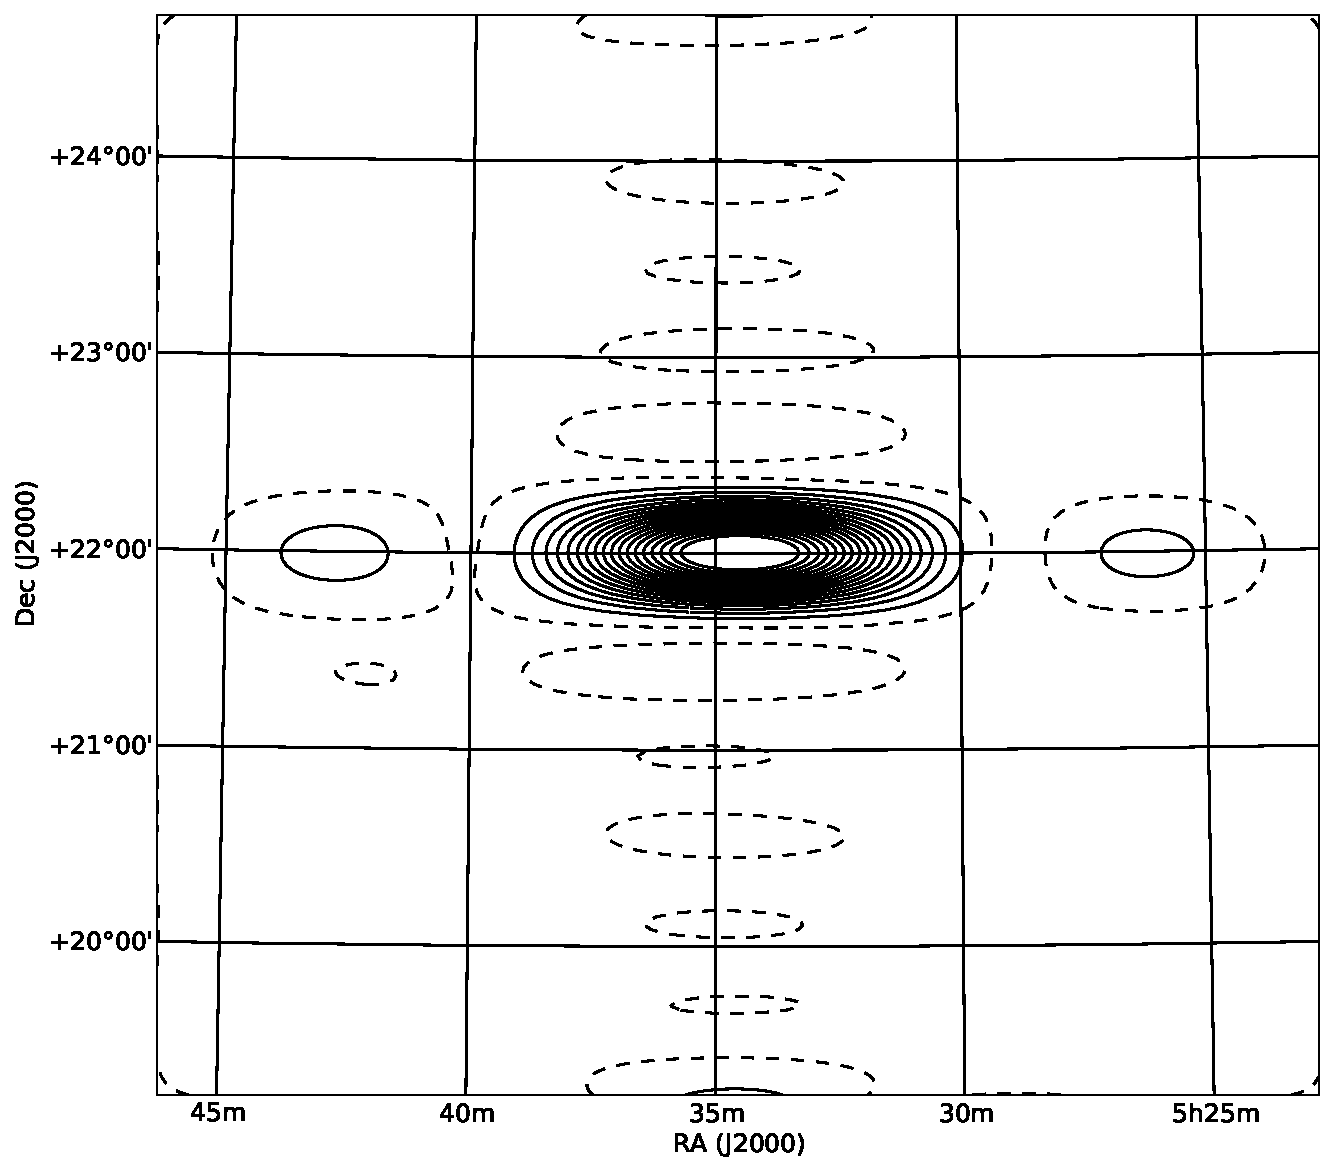
\includegraphics[scale=0.3]{{graphics/fx/corr.2455996.22803.tau.s.ms.natural.CORRECTED_DATA.channel.1ch}.pdf}
    \label{fig:fx_tau_natural}
    }
    \hspace{10pt}
    \subfloat[Dirty image with uniform weighting of the point source Taurus A.]{
    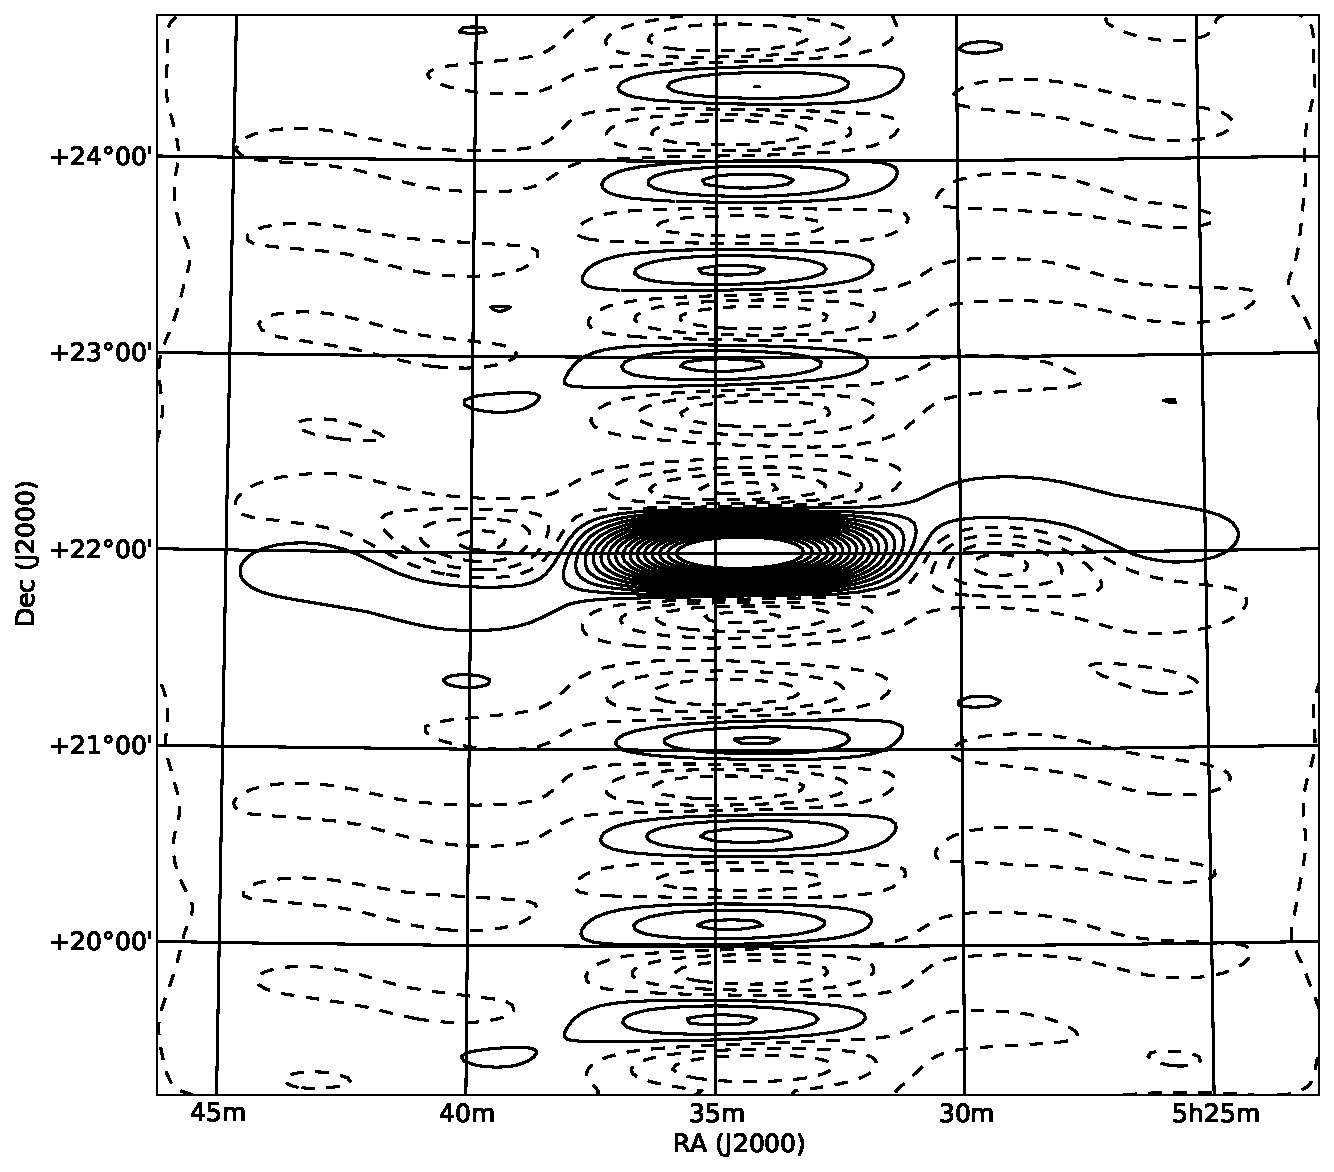
\includegraphics[scale=0.3]{{graphics/fx/corr.2455996.22803.tau.s.ms.uniform.CORRECTED_DATA.channel.1ch}.pdf}
    \label{fig:fx_tau_uniform}
    }
    
    \label{fig:fx_weighting}
    \caption{
    }
\end{figure}

\subsection{Spatial FFT Results}
\label{sfft results}

%beam crossing/imaging/beamformer

%conversion to baselines
The output image data from the spatial FFT can be converted to uv sampled baselines by performing an inverse FFT.
All redundant baselines are combined into a single unique baseline which makes pre-measurement calibration essential to producing a good observable.
In total 52 unique baselines are produced along with the auto correlation.
Each unique spatial FFT baseline is a linear combination of antenna pair baselines at the same uv position.
Once in the baseline correlation format the same pipeline that is used for the FX correlator is used to convert the data into measurement sets.

%dirty/clean images
Antenna gain calibration can not be performed on the spatial FFT correlations since each baseline is made up of a linear combination of redundant baselines.
Thus no calibration is applied to the output data.
The flux scale is set by using the flux scale from the FX images.
This scale can be set during the observation or in post processing since it is a baseline independent amplitude scaling.

\begin{figure}
    \centering

    \subfloat[Dirty image of Taurus formed from the spatial FFT imagers, the flux scale(Jy) has been fixed to the scale based on the same image from the FX correlator.]{
    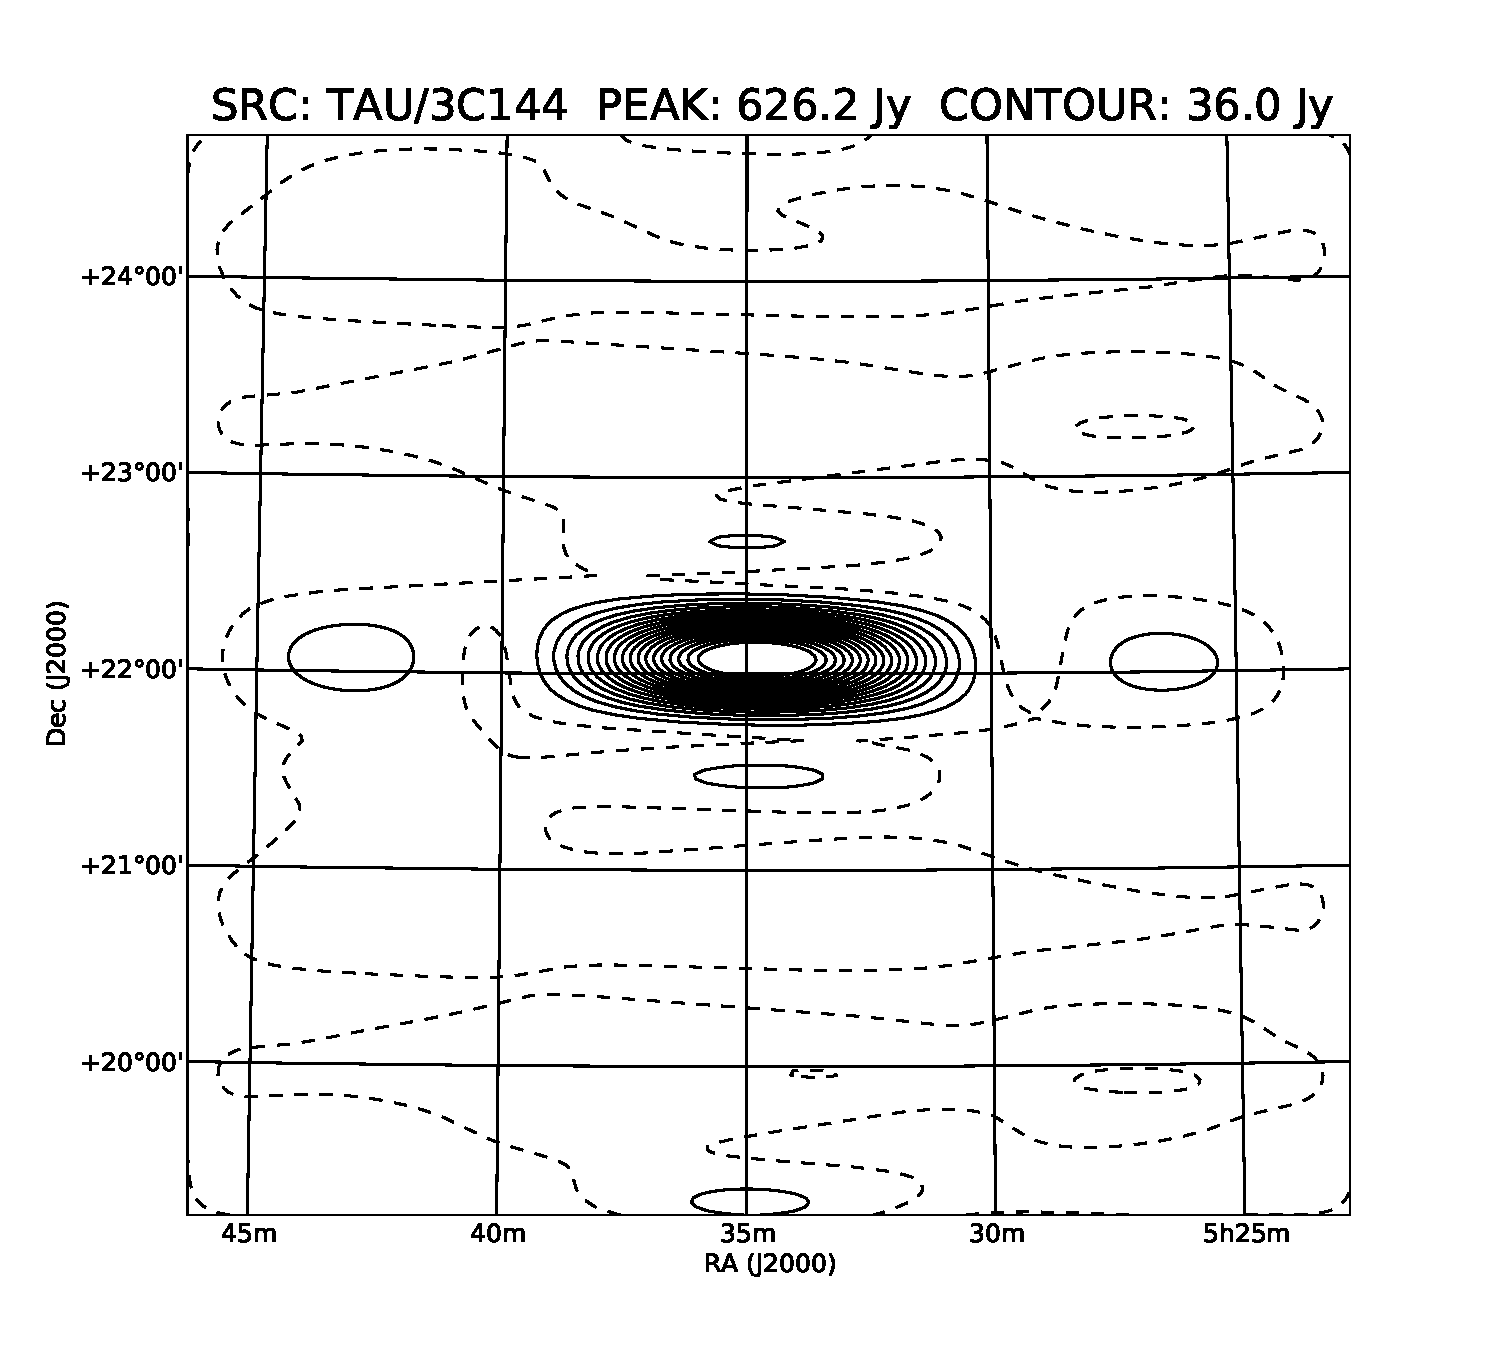
\includegraphics[scale=0.3]{{graphics/sfft/img.2455996.22807.tau.s.ms.DATA.channel.1ch}.pdf}
    \label{fig:sfft_tau_dirty}
    }
    \hspace{10pt}
    \subfloat[Cleaned image of the Taurus field.]{
    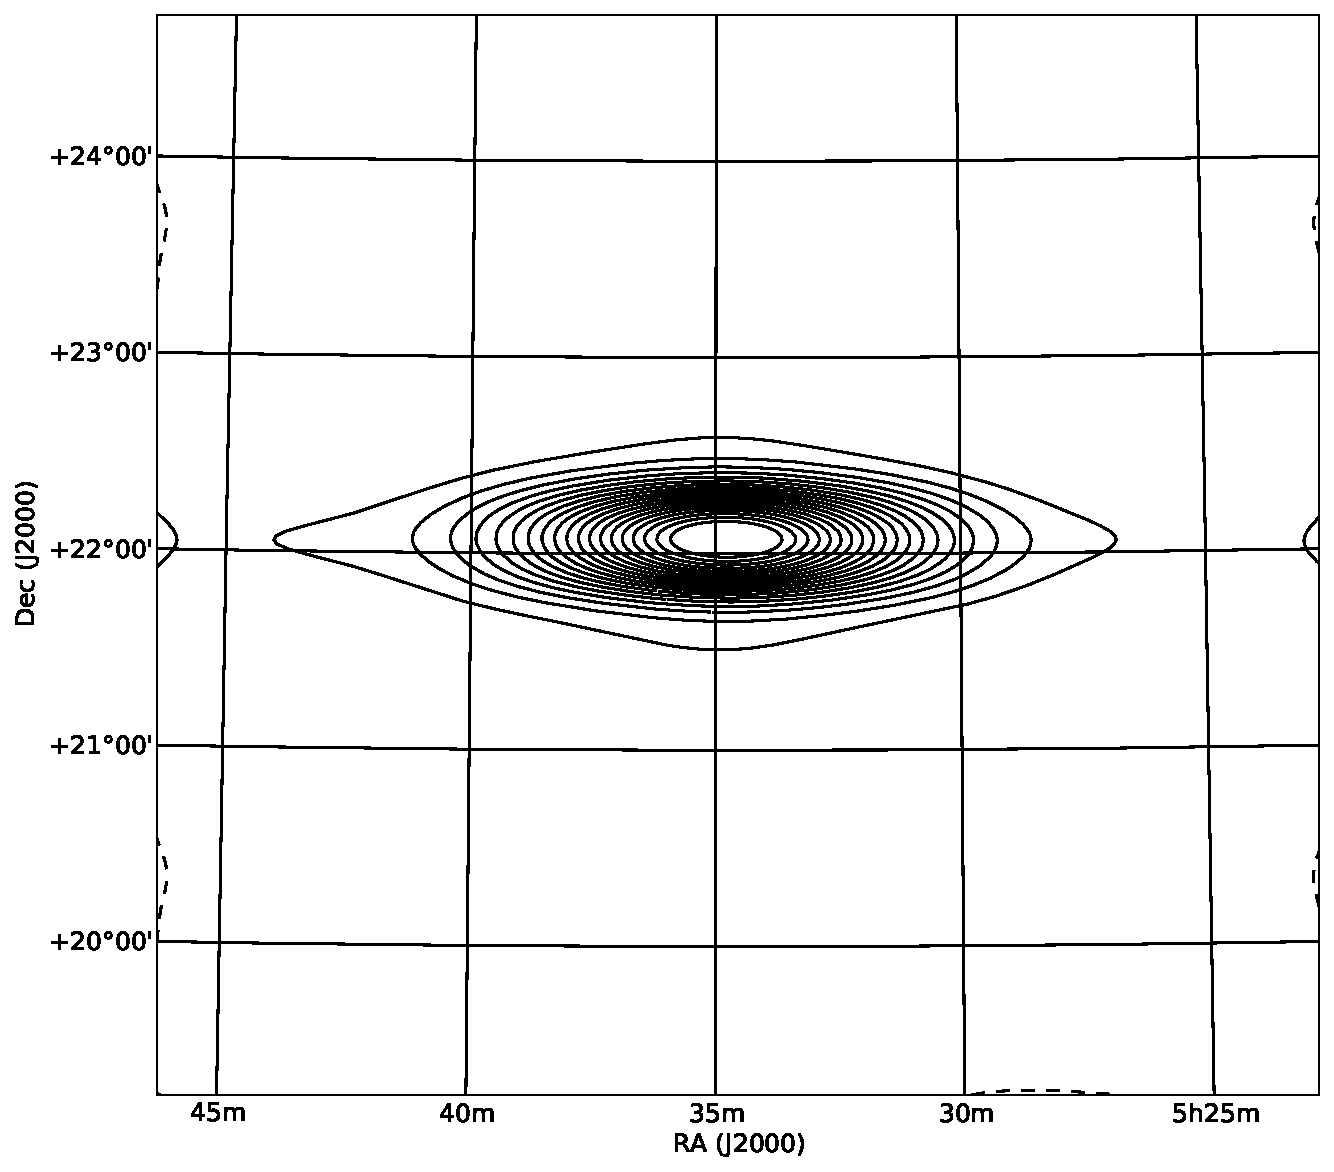
\includegraphics[scale=0.3]{{graphics/sfft/img.2455996.22807.tau.s.ms.DATA.channel.1ch.restored}.pdf}
    \label{fig:sfft_tau_clean}
    }
    
    \label{fig:sfft_tau}
    \caption{The images produced by the spatial FFT imager are comparable in noise and dynamic range to those produced with calibrated FX correlator data.
    }
\end{figure}

\subsection{Comparison of FX Correlator and Spatial FFT}

In the ideal case, observations using the spatial FFT will be identical to observations using an FX correlator.

%calibration variation
%images: 3c48 dirty/clean
%images: cas + sun
%baselines: fx,avg,mdl,sfft
%error analysis

\section{Discussion}
\label{discussion}

%what has been accomplished
%further work on SFFT calibration
%uses: space debris, transient detection/pulsars

\bibliography{refs}{}
\bibliographystyle{mn2e}

\end{document}
